\documentclass[11pt, a4paper]{article}
\usepackage[utf8]{inputenc}
\usepackage{amsmath,setspace,geometry}
\usepackage{amsthm}
\usepackage{amsfonts}
\usepackage{mathtools}
\mathtoolsset{showonlyrefs}
\usepackage[shortlabels]{enumitem}
\usepackage{rotating}
\usepackage{pdflscape}
\usepackage{graphicx}
\usepackage{bbm}
\usepackage[dvipsnames]{xcolor}
\usepackage[colorlinks=true, linkcolor= RawSienna, citecolor = RawSienna, filecolor = RawSienna, urlcolor = RawSienna, hypertexnames = true, backref = page]{hyperref}
\usepackage[]{natbib} 
\bibpunct[:]{(}{)}{,}{a}{}{,}
\geometry{left = 1.0in,right = 1.0in,top = 1.0in,bottom = 1.0in}
\usepackage[english]{babel}
\usepackage{float}
\usepackage{caption}
\usepackage{subcaption}
\usepackage{tikz}
\usepackage{booktabs}
\usepackage{pdfpages}
\usepackage{threeparttable}
\usepackage{framed}
\usepackage{comment}
\usepackage{lscape}
\usepackage{bm}
\setstretch{1.3}
%\usepackage[tablesfirst,nolists]{endfloat}

\usepackage[T1]{fontenc}
\usepackage{mlmodern}  % 太いComputer Modern
% MLmodernのバグを修正: cf. https://tex.stackexchange.com/questions/646333/size-of-integral-symbol-in-section-header-with-mlmodern
\DeclareFontFamily{OMX}{mlmex}{}
\DeclareFontShape{OMX}{mlmex}{m}{n}{<->mlmex10}{} 
\usepackage{tgtermes} % 数式以外の欧文をTXフォントで上書き

\newtheorem{theorem}{Theorem}
\newtheorem{assumption}{Assumption}
\newtheorem{lemma}{Lemma}
\newtheorem{definition}{Definition}
\newtheorem{proposition}{Proposition}
\newtheorem{claim}{Claim}
\newtheorem{corollary}{Corollary}
\newtheorem{example}{Example}
\DeclareMathOperator{\rank}{rank}

\theoremstyle{remark}
\newtheorem{remark}{Remark}

\title{Note on Conduct Parameter Approach in Empirical Industrial Organization}
\author{Yuri Matsumura\thanks{\href{mailto:}{yuri.matsumura23@gmail.com}, Department of Economics, Rice University.} \and Suguru Otani \thanks{\href{mailto:}{suguru.otani@e.u-tokyo.ac.jp}, Market Design Center, Department of Economics, University of Tokyo
\\Declarations of interest: none %this is for Economics Letters
}}

\begin{document}

\maketitle
\begin{abstract}
    TBA
\end{abstract}

\noindent\textbf{Keywords:} Conduct parameters, Homogenous Goods Market, Mathematical Programming with Equilibrium Constraints, Monte Carlo simulation
\vspace{0in}
\newline
\noindent\textbf{JEL Codes:} C5, C13, L1

\bigskip





\section{Introduction}
Measuring competitiveness is an important task in the empirical industrial organization literature.
A conduct parameter is considered to be a useful measure of competitiveness. 
However, the parameter cannot be directly measured from data because data generally lack information about marginal costs.
Therefore, researchers endeavor to identify and estimate conduct parameters.


In homogeneous goods markets, \citet{bresnahan1982oligopoly} proposes an approach to identify a conduct parameter using demand rotation instruments under the linear demand and linear marginal cost model.
This result is extended to nonlinear cases by \citet{lau1982identifying}.

In this paper, we revisit the identification problem in homogeneous goods markets.
We show that the identification result in \citet{lau1982identifying} is incorrect.

















\section{Model}
Consider a homogeneous product market where a representative firm maximizes its profit, given by the function:
\begin{align}
    \Pi = P(Q)Q - C(Q),
\end{align}
where $P(Q)$ represents the aggregate inverse demand function, and $C(Q$ is the aggregate cost function.
Assume that the demand function is decreasing in $Q$, $P'(Q) \equiv \frac{dP}{dQ} < 0$ and the cost function is increasing in $Q$, $C'(Q) \equiv \frac{dC}{dQ} > 0$.

To determine the optimal quantity (or equilibrium quantity), the firm adjusts the quantity such that the marginal gain from increasing the quantity equals the marginal loss. 
However, the firm recognizes only a fraction of the marginal gain, denoted by $\theta \in [0,1]$. 
As a result, the equilibrium condition can be written as:
\begin{align}
    \theta P'(Q)Q = - (P(Q) - MC(Q)),
\end{align}
where $MC(Q)$ represents the marginal cost of production.
The left hand is the marginal gain by increasing price and the right hand represents the marginal loss.
By rewriting the relationship, we have
\begin{align}
    P(Q)+ \theta P'(Q)Q = MC(Q). \label{eq:optimality_conditition}
\end{align}
The equilibrium quantity is also given by the solution to \eqref{eq:optimality_conditition}.
This relationship is easy to interpret when $\theta = 1$ because it corresponds to the first-order condition of a monopoly firm.
Additionally, depending on the value of $\theta$, the relation can nest the first-order condition of other models such as perfect competition ($\theta=0$) and Cournot competition ($\theta=1/N$). See \citet{adachiMicrofoundation2023} for the detail of the interpretation.


\subsection{Conjectural Variation Model}



The foundation of the conduct parameter approach is a conjectural variation model.

Conjectural variation how competitors react to the change in the firm's output.
For example, in a homogeneous product market, the conjectural variation is defined as
\begin{align}
    r_{ij}(q_i) \equiv \frac{\partial q_j}{\partial q_i}.
\end{align}
Consider a firm $i$'s profit function
\begin{align}
    \pi_i = P(Q)q_i - C(q_i),
\end{align}
where $Q = \sum_{j=1}^N q_j$ is the aggregate output.
Given the conjectural variation, the firm's first-order condition is given by
\begin{align}
    P(Q) + P'(Q)(1+r_{ij}(q_i))q_i = MC(q_i).
\end{align}
Then, the conduct parameter is equivalent to the term $1+r_{ij}(q_i)$ in the first-order condition.
This conjectural variation model nests several competition models such as Cournot $r_{ij}(q_i) = 0$ and Bertrand $r_{ij}(q_i) = -1$.

However, this conjectural variation model has been criticized by several papers.
As an example, let's consider the Cournot conjecture.
In this conjecture, each firm believes that its competitors does not react to the change in its output.
Then, the first-order condition is given by
\begin{align}
    P(Q) + P'(Q)q_i = MC(q_i).
\end{align}
Then, under appropriate assumptions on the inverse demand function and the marginal cost function, by applying the implicit function theorem to the first-order condition, the derivative of reaction function $q_i = \rho_i(q_{-i})$ with respect to $q_j$ is given by
\begin{align}
    \frac{\partial \rho_i}{\partial q_j} = -\frac{q_iP''(Q) + P'(Q)}{P'(Q) + q_iP''(Q)+ P'(Q) - mc'_i(q_i)}.
\end{align}

Assume that the inverse demand function is linear and the marginal cost is constant: 
$P'(Q) \ne 0$, $P''(Q) = 0$ and $MC'(q_i) = 0$.
Then, the derivative of reaction function is given by
\begin{align}
    \frac{\partial \rho_i}{\partial q_j} = \frac{P'(Q)}{2P'(Q)} = \frac{1}{2}.
\end{align}
When the market is duopoly, this implies that $\rho'_{j}(q_i) = \frac{1}{2}$.
However, this contradicts the conjecture that the firm does not react to the change in its output, that is, $\rho'_{j}(q_i) \ne r_{ij}(q_i)$.
This is a well-known inconsistent result in the Cournot conjecture.
In other words, firms' beliefs about the reaction to the change in output are not consistent with the reaction in equilibrium.

To solve the inconsistency, proposes a new equilibrium concept called consistent conjectures equilibrium.


\begin{framed}
    \begin{definition}
        A consistent conjectures equilibrium is a pair of the equilibrium quantity $q^*$ and the conjectural variation $r_i = (r_{i1}(q_i), \ldots, r_{iN}(q_i))$ that satisfies 
        \begin{align}
            q^*_i = \rho_i(q_{-i}^*),
        \end{align}
        where $q_{-i}^*$ is the equilibrium quantity of the other firms, and there is $\varepsilon > 0$ such that
        \begin{align}
            r_{ij}(q_j^*) = \frac{\partial \rho_{i}(q_{-i}^*)}{\partial q_j^*},\quad q^*_{i} - \varepsilon < q_i < q^*_{i} + \varepsilon.
        \end{align}
        for all $i$.
    \end{definition}
\end{framed}























\section{Identification}
Now, consider an econometric model of the above model.
Define the aggregate inverse demand and aggregate marginal cost function as $P(Q, X^{d})$ and $MC(Q, X^{s})$ where $X^{d}$ and $X^{s}$ are the vector of exogenous variables.
Assume that $X^{d}$ and $X^{s}$ are exclusive, that is, there is no common variable in $X^{d}$ and $X^{s}$.
Thus, $X^{d}$ works as demand shifters and $X^{s}$ works as cost shifters. 
Suppose that the researcher observes the aggregate price $P$ and the aggregate quantity $Q$, and the vector of exogenous variables $X^{d}$ and $X^{s}$.
In this setting, the researcher can independently identify the inverse demand function by using the demand and cost shifters.

Therefore, the researcher wants to identify the conduct parameter $\theta$ and the marginal cost function $MC(Q, X^{s})$ from the observed data.
\cite{bresnahan1982oligopoly} considers the identification of the conduct parameter and the marginal cost function in linear demand and linear marginal cost model.
Here, the identification problem is reduced to the identification of the conduct parameter and the parameters of the marginal cost function.
\citet{bresnahan1982oligopoly} discusses that when the researcher can obtain a demand shifter $Z$, called demand rotation instrument, that changes the slope and intercept of the inverse demand function, the conduct parameter and the marginal cost parameter can be identified, and \citet{matsumura2023resolving} provides a detailed condition for the identification.


Obviously, the setting considered in \citet{bresnahan1982oligopoly} is a very limited case.
\citet{lau1982identifying} considers the identification problem in a more general setting.
Instead of directly proving identification, \citet{lau1982identifying} takes an indirect approach by specifying the conditions under which the model is not identified. 
The definition of non-identification is as follows:
\begin{framed}
    \begin{definition}\label{def:non_identification}
    Non-identification implies for any $X^{d}$ and $X^{s}$,
    \begin{align}
    P(Q^e, X^{d}) + \theta \frac{\partial P}{\partial Q}(Q^e, X^{d})Q^e &= MC(Q^e, X^{s}),  \label{eq:foc_alpha}\\
    P(Q^e, X^{d}) + \theta^{*} \frac{\partial P}{\partial Q}(Q^e, X^{d})Q^e &= MC^{*}(Q^e, X^{s}),\label{eq:foc_beta}
    \end{align}
    where $\theta \neq \theta^{*}$, $MC \ne MC^{*}$,\footnote{This condition is not stated in \citet{lau1982identifying}, but assuming $MC = MC^{*}$ makes the identification simple.} and the equilibrium quantity $Q^e$ has a reduced form functions $Q^e = h(X^{d}, X^{s})$ and $Q^e = h^{*}(X^{d}, X^{s})$ defined by \eqref{eq:foc_alpha} and \eqref{eq:foc_beta} respectively are identical.
    \end{definition}
\end{framed}
In other words, given two distinct pairs of conduct parameter and marginal cost, the equilibrium quantity $Q^e$ solves the first-order condition for both pairs.
Note that \eqref{eq:foc_alpha} and \eqref{eq:foc_beta} are referred as "supply equation" in \citet{bresnahan1982oligopoly}.
Non-identification asks the following question: given an identified inverse demand function $P(Q, X^{d})$, is it possible to find two distinct pairs of conduct parameter and marginal cost, $(\theta, MC)$ and $(\theta^{*}, MC^{*})$, that lead to observable equivalent equilibrium?
Note that the marginal cost function need to be nonparametrically identified; that is, the researcher needs to identify the marginal cost without any assumption on the functional form.

\citet{lau1982identifying} finds that separability of the inverse demand function and non-identification are equivalent.
\begin{framed}
\begin{theorem}\label{theorem_lau}
    Under the assumption that the industry inverse demand and cost functions are twice continuously differentiable, the index of competitiveness $\theta$ cannot be identified from data on industry price and output and other exogenous variables alone if and only if the industry inverse demand function is separable in $X^{d}$, that is,
    \begin{align}
        p = P(Q, r(X^{d})), \label{eq:demand_separable}
    \end{align}
    but not take the form, 
    \begin{align}
        P = Q^{-1/\theta}r(X^{d}) + s(Q). \label{eq:identification_separable}
    \end{align}
\end{theorem}
\end{framed}
The theorem implies that the conduct parameter is identified when the demand function is not separable, except \eqref{eq:identification_separable}.

\begin{comment}
    \citet{bresnahan1982oligopoly} considers a model with linear demand and marginal cost.
    He considers a demand function such that $P = \alpha_0 + (\alpha_1 + \alpha_2 Z) Q + \alpha_3 Y + \alpha_4 Z  + \varepsilon$ where $Z$ is called a demand rotation instrument.
    It is easy to verify that this demand is not separable.
    Under the demand, the conduct parameter and the marginal cost parameter can be identified.
    \citet{matsumura2023resolving} provide more detailed conditions for the identification.
\end{comment}


\section{Summary of Goldman and Uzawa (1964)}
Before investigating the proof of Lau, we introduce results in \citet{goldmanNote1964}, which Lau also relies on.
\citet{goldmanNote1964} consider the following setting.
Let $n$ be the number of variables and $x = (x_{1},\ldots, x_{n})$ be a vector of $n$ variables.
Consider a partition of $X$ into $K$ parts, $\{x^1, \ldots, x^K\}$ such that $X = \bigcup_{k=1}^K x^k$ and $x^k \cap x^l = \emptyset$ for $k\ne l$.
\begin{framed}
    \begin{definition}\label{def:weal_separable}
        A function is weakly separable with respect to the partition if 
        \begin{align}
            \frac{\partial}{\partial x_l}\left(\frac{\frac{\partial f}{\partial x_i}(x^1, \ldots, x^K)}{\frac{\partial f}{\partial x_j}(x^1, \ldots, x^K)}\right) = 0, \quad i,j\in x^k, l \notin x^k.
        \end{align}
    \end{definition}
\end{framed}
This implies that the ratio of the derivative with respect to $x_i$ and $x_j$, which are in the same category, is not affected by the change in the variables in other partitions.
Intuitively, by taking the ratio, the component of $f$ relating to $x_l$ is canceled out, and hence the derivative of the ratio with respect to $x_l$ becomes zero.
When $f$ is a utility function, this implies that the marginal rate of substitution between commodity $i$ and $j$ in the same partition is independent of the quantities of commodities outside $x^k$.

Then, \citet{goldmanNote1964} specifies the functional form that a weak separable function should satisfy.
\begin{framed}
    \begin{theorem}\label{thorem_2_GU}
    A function $f(x)$ is weakly separable with respect to a partition $\{x^1, .. ., x^K\}$ if and only if $f(x)$ is of the form: 
    \begin{align}
        f(X) = \Phi(r^1(x^{1}),\ldots, r^K(x^{K})   )
    \end{align} where $\Phi(r^1,\ldots, r^K)$ is a function of $K$ variables and, for each $k$, $r^k(x^{k})$ is a function subvector $x^{k}$ alone.
    \end{theorem}
\end{framed}


Let $\{Q,X_{1}^{d}, \ldots,  X_{K_d}^{d}\}$ be a vector of variables where $K_d$ is the dimension of $X^{d}$.
Consider a partition $\{Q, X^{d}\}$, and let $r^1(Q) = Q$.
Then, $P(Q, r(X^{d}))$ satisfies the form in Theorem \ref{thorem_2_GU}.
Therefore, the definition of separable function in Theorem \ref{theorem_lau} corresponds to the functional form in  Theorem \ref{thorem_2_GU}, which implies that the separability in \citet{lau1982identifying} corresponds to the weak separability in \citet{goldmanNote1964}.

\begin{remark}
    The linear demand function in \citet{bresnahan1982oligopoly} is not separable:
    \begin{align}
        \frac{f_Z}{f_Y} = \frac{\alpha_2 Q}{\alpha_3} \Longrightarrow \frac{\partial P_Z/f_Y}{\partial Q} = \frac{\alpha_2}{\alpha_3} \ne 0,
    \end{align}
    where $\alpha_2/\alpha_3 \ne 0$ comes from the sufficient condition for the identification in \citet{matsumura2023resolving}.
    \qed
\end{remark}


The next lemma is a key lemma in the proof of \citet{lau1982identifying}.
\begin{framed}
\begin{lemma}\label{lemma_1_GU}
    Let $f(x)$ and $g(x)$ be two continuously twice-differentiable functions of $n$ variables $x=(x_1, \dots, x_n)$. If each indifference surface is connected, and if there exists a function $\lambda(x)$ such that
    \begin{align}
    \frac{\partial f}{\partial x_i}(x) &= \lambda(x)\frac{\partial g}{\partial x_i}(x), \quad i=1, \dots, n, \quad \text{for all } x, \label{eq:transform_f}
    \end{align}
    then $f(x)$ is a transformation of $g(x)$; namely, there exists a function $T(\cdot)$ of one variable such that
    \begin{align}
    f(x) &= T(g(x)) \quad \text{for all } x.
    \end{align}
    Hence, in particular, the function $\lambda(x)$ satisfying \eqref{eq:transform_f} must be of the form:
    \begin{align}
        \lambda(x) &= \Lambda(g(x)) \quad \text{for all } x, \label{eq:form_of_lambda}
    \end{align}
    with some function $\Lambda(\cdot)$ of one variable.
\end{lemma}
\end{framed}
If there is a function $T$ such that $f(x) = T(g(x))$, then by the chain rule, we have $\frac{\partial f}{\partial x_i}(x) = T'(g(x))\frac{\partial g}{\partial x_i}(x)$ where $T'$ is the derivative of $T$.
Thus, by defining $\lambda(x) = T'(g(x))$, we have $\frac{\partial f}{\partial x_i}(x) = \lambda(x)\frac{\partial g}{\partial x_i}(x)$.
Intuitively, the lemma implies that the converse of the chain rule holds under additional conditions.


\section{Necessity Proof in Lau(1982)}\label{sec:proof_lau_necessity}
Now, let's investigate the proof of \citet{lau1982identifying}.
We try to fill some gaps between the lines in the original proof.
First, we show that the non-identification implies that the inverse demand function is separable.

Suppose that $(\theta, MC)$ is the pair of the true model component, but there is another pair $(\theta^{*}, MC^{*})$ that leads to an observable equivalent equilibrium.
Given $X^{d}$ and $X^{s}$, the true component $(\theta, MC)$ satisfy the first-order condition for the equilibrium quantity $Q^e$,
\begin{align}
    F(Q^e, X^{d}, X^{s}) \equiv P(Q^e, X^{d}) + \theta\frac{\partial P}{\partial Q}(Q^e, X^{d})Q^e - MC(Q^e, X^{s}) = 0.
\end{align}
Assume that the derivative of $F$ with respect to $Q$ at the equilibrium quantity $Q^e$ is nonzero;
\begin{align}
    \frac{\partial F}{\partial Q}(Q^e, X^{d}, X^{s}) = (1+\theta)\frac{\partial P}{\partial Q}(Q^e, X^{d}) + \theta\frac{\partial^2 P}{\partial Q^2}(Q^e, X^{d})Q^e - \frac{\partial MC}{\partial Q}(Q^e, X^{s}) \ne 0.
\end{align}
Then, we can apply the implicit function theorem, and for the reduced-form equation $Q^e = h(X^{d}, X^{s})$, the derivatives of $F$ for each variable are
\begin{align}
    \frac{\partial F}{\partial X^{d}_i}(Q^e, X^{d}, X^{s}) & =  \frac{\partial P}{\partial X^{d}_{i}}(Q^e, X^{d}) + \theta\frac{\partial^2 P}{\partial X^{d}_{i}\partial Q}(Q^e, X^{d})Q^e,\\
    \frac{\partial F}{\partial X^{s}_i}(Q^e, X^{d}, X^{s}) & =  -\frac{\partial MC}{\partial X^{s}_{i}}(Q^e, X^{s}),\\
    \frac{\partial F}{\partial Q}(Q^e, X^{d}, X^{s}) & = (1+\theta)\frac{\partial P}{\partial Q}(Q^e, X^{d}) + \theta\frac{\partial^2 P}{\partial Q^2}(Q^e, X^{d})Q^e - \frac{\partial MC}{\partial Q}(Q^e, X^{s}).
\end{align}
Then, the derivative of $h$ with respect to the demand shifter and the cost shifters are
\begin{align}
    \frac{\partial h}{\partial X^{d}_{i}}(X^{d}, X^{s}) = -\frac{\frac{\partial P}{\partial X^{d}_{i}}(Q^e, X^{d}) + \theta\frac{\partial^2 P}{\partial X^{d}_{i}\partial Q}(Q^e, X^{d})Q^e }{(1+\theta)\frac{\partial P}{\partial Q}(Q^e, X^{d}) + \theta\frac{\partial^2 P}{\partial Q^2}(Q^e, X^{d})Q^e - \frac{\partial MC}{\partial Q}(Q^e, X^{s})}, \label{eq:foc_derivative_demand}
\end{align}
and
\begin{align}
    \frac{\partial h}{\partial X^{s}_{i}}(X^{d}, X^{s}) & = \frac{\frac{\partial MC}{\partial X^{s}_{i}}(Q^e, X^{s})}{(1+\theta)\frac{\partial P}{\partial Q}(Q^e, X^{d}) + \theta\frac{\partial^2 P}{\partial Q^2}(Q^e, X^{d})Q^e - \frac{\partial MC}{\partial Q}(Q^e, X^{s})}. \label{eq:foc_derivative_supply}
\end{align}
By applying the same argument for \eqref{eq:foc_beta}, we obtain 
\begin{align}
    \frac{\partial h^{*}}{\partial X^{d}_{i}}(X^{d}, X^{s}) &= -\frac{\frac{\partial P}{\partial X^{d}_{i}}(Q^e, X^{d}) + \theta^{*}\frac{\partial^2 P}{\partial X^{d}_{i}\partial Q}(Q^e, X^{d})Q^e }{(1+\theta^{*})\frac{\partial P}{\partial Q}(Q^e, X^{d}) + \theta^{*}\frac{\partial^2 P}{\partial Q^2}(Q^e, X^{d})Q^e - \frac{\partial MC^{*}}{\partial Q}(Q^e, X^{s})}, \\
    \frac{\partial h^{*}}{\partial X^{s}_{i}}(X^{d}, X^{s}) & = \frac{\frac{\partial MC^{*}}{\partial X^{s}_{i}}(Q^e, X^{s})}{(1+\theta^{*})\frac{\partial P}{\partial Q}(Q^e, X^{d}) + \theta^{*}\frac{\partial^2 P}{\partial Q^2}(Q^e, X^{d})Q^e - \frac{\partial MC^{*}}{\partial Q}(Q^e, X^{s})}.
\end{align}

 
% Use the definition of non-identification
As the non-identification implies that $Q^e = h(X^{d}, X^{s}) = h^{*}(X^{d}, X^{s})$ for all $X^{d}$ and $X^{s}$, we must have
\begin{align}
    \frac{\partial h^{*}}{\partial X^{d}_{i}}(X^{d}, X^{s})  = \frac{\partial h}{\partial X^{d}_{i}}(X^{d}, X^{s}), \text{  and  } \frac{\partial h^{*}}{\partial X^{s}_{i}}(X^{d}, X^{s})  = \frac{\partial h}{\partial X^{s}_{i}}(X^{d}, X^{s}), \quad \forall X^{d}, X^{s}. \label{eq:observale_equivalence_derivative}
\end{align}
Thus, we obtain 
\begin{align}
    & \frac{\frac{\partial P}{\partial X^{d}_{i}}(Q^e, X^{d}) + \theta^{*}\frac{\partial^2 P}{\partial X^{d}_{i}\partial Q}(Q^e, X^{d})Q^e }{(1+\theta^{*})\frac{\partial P}{\partial Q}(Q^e, X^{d}) + \theta^{*}\frac{\partial^2 P}{\partial Q^2}(Q^e, X^{d})Q^e - \frac{\partial MC^{*}}{\partial Q}(Q^e, X^{s})}\\
    &\hspace{1cm} = - \frac{\frac{\partial P}{\partial X^{d}_{i}}(Q^e, X^{d}) + \theta \frac{\partial^2 P}{\partial X^{d}_{i}\partial Q}(Q^e, X^{d})Q^e }{(1+\theta)\frac{\partial P}{\partial Q}(Q^e, X^{d}) + \theta\frac{\partial^2 P}{\partial Q^2}(Q^e, X^{d})Q^e - \frac{\partial MC}{\partial Q}(Q^e, X^{s})}, \label{eq:derivative_q_x_d}
\end{align}
and
\begin{align}
    &\frac{\frac{\partial MC^{*}}{\partial X^{s}_{i}}(Q^e, X^{s})}{(1+\theta^{*})\frac{\partial P}{\partial Q}(Q^e, X^{d}) + \theta^{*}\frac{\partial^2 P}{\partial Q^2}(Q^e, X^{d})Q^e - \frac{\partial MC^{*}}{\partial Q}(Q^e, X^{s})}\\ 
    &\hspace{1cm} = \frac{\frac{\partial MC}{\partial X^{s}_{i}}(Q^e, X^{s})}{(1+\theta)\frac{\partial P}{\partial Q}(Q^e, X^{d}) + \theta\frac{\partial^2 P}{\partial Q^2}(Q^e, X^{d})Q^e - \frac{\partial MC}{\partial Q}(Q^e, X^{s})}.\label{eq:derivative_q_x_s}
\end{align}


From \eqref{eq:derivative_q_x_s}, Lau states that there is a relationship between $MC$ and $MC^{*}$ defined as
\begin{align}
    \frac{\partial MC^{*}}{\partial X^{s}_{i}}(Q^e, X^{s}) = \lambda(Q^e, X^{s})\frac{\partial MC}{\partial X^{s}_{i}}(Q^e, X^{s}), \quad \forall Q^e, X^{s}. \label{eq:derivative_q_x_s_la}
\end{align}
Note that in the original paper, Lau does not use $Q^e$ but $Q$, which can be regarded as not the equilibrium quantity but just a quantity.
However, in footnote 5, Lau recognizes that $Q$ is a function of $X^{d}$ and $X^{s}$, and hence we use $Q^e$ in our definition to express that we are considering the equilibrium quantity.

By applying Lemma \ref{lemma_1_GU} to this, he obtains
\begin{align}
    MC^{*}(Q^e, X^{s}) = T\left(MC(Q^e, X^{s}), Q^e\right), \quad \forall Q^e, X^{s}, \label{eq:transformation_T_mc_la}
\end{align}
and by substituting the left-hand side of \eqref{eq:foc_alpha} and \eqref{eq:foc_beta}, he obtains 
\begin{align}
    P(Q^e, X^{d}) + \theta^{*} \frac{\partial P}{\partial Q}(Q^e, X^{d}) Q^e & = T\left(P(Q^e, X^{d}) + \theta \frac{\partial P}{\partial Q}(Q^e, X^{d}) Q^e, Q^e\right), \quad \forall Q^e, X^{d}.\label{eq:transformation_T_demand_la}
\end{align}
After obtaining \eqref{eq:transformation_T_demand_la}, Lau considers two cases where $X^{d}$ is a scalar and where $X^{d}$ is not a scalar.

\subsection{Case 1: The demand shifter is a scalar}

As for the scalar case, based on the notation and the equation numbers in our setting, Lau states the following:
\begin{quote}
    "If $X^{d}$ is a scalar, then for any given $\theta^*$, the left-hand side of \eqref{eq:transformation_T_demand_la} is a function of $Q^e$ and $X^{d}$.  
    The right-hand side is a function of two independent variables, $P(Q^e, X^{d}) + \theta \frac{\partial P}{\partial Q}(Q^e, X^{d}) Q^e,$ and $Q^e$.  
    If the transformation between these two alternative sets of independent variables is non-singular, there always exists a $T(\cdot, Q^e)$ such that \eqref{eq:transformation_T_demand_la} holds.
    The transformation becomes singular only if,
    \begin{align}
        \frac{\partial P}{\partial X^{d}}(Q, X^{d}) + \theta^{*} \frac{\partial^2 P}{\partial X^{d}\partial Q}(Q, X^{d})Q = 0. \label{eq:singular_equation}
    \end{align}
    which can be integrated to yield
    \begin{align}
        P(Q, X^{d}) = Q^{-\frac{1}{\theta}}r(X^{d}) + s(Q).
    \end{align}
    Thus, except for this singular case, $\theta$ cannot be uniquely identified when $X^{d}$ is a scalar."
\end{quote}
This is a key argument in Lau's paper.
When $X^{d}$ is a scalar, we can identify $\theta$ only when the inverse demand function is given by \eqref{eq:identification_separable}.
Additionally, when $\theta = 0$, the inverse demand function is not well-defined, and hence we cannot identify $\theta$ when the true conduct is perfect competition.

The intuition of singular case is as follows.
When \eqref{eq:singular_equation} holds, the numerator in the right-hand side of \eqref{eq:derivative_q_x_d} is zero while the numerator in the left-hand side is not zero in general.\footnote{See \ref{app:ommitted_proof} for the detailed discussion.}
Thus, observable equivalence is immediately violated; $\frac{\partial h}{\partial X^{d}_{i}}(X^{d}, X^{s}) \neq \frac{\partial h^{*}}{\partial X^{d}_{i}}(X^{d}, X^{s})$ for any $X^{d}$ and $X^{s}$.
Therefore, we can not transform the first-order condition under the true component $(\theta, MC)$ into the first-order condition under $(\theta^*, MC^*)$ through $T$ while keeping the equilibrium quantity the same.

\subsubsection{Is the differential equation necessary for the transformation to be singular?}

An important concern is that \eqref{eq:singular_equation} is just a sufficient condition for $T$ to be singular, but cannot be the necessary condition.
To see this, we first show the necessary condition for the existence of $T$.
For notional simplicity, define a function
\begin{align}
    MR(Q, X^{d}; \theta) \equiv P(Q, X^d) + \theta \frac{\partial P}{\partial Q}(Q, X^d) Q.
\end{align}
Suppose that there exists a transformation $T$ such that
\begin{align}
    MR(Q, X^{d}; \theta^{*}) = T(MR(Q, X^{d}; \theta)).
\end{align}
Let $(Q_1, X_1)$ and $(Q_2, X_2)$ be different combinations of $(Q,X^{d})$ where $Q_1 \ne Q_2$ and $X_1 \ne X_2$.
The existence of transformation $T$ requires that
\begin{align}
    MR(Q_1, X_1; \theta) = MR(Q_2, X_2; \theta) \text{ implies } MR(Q_1, X_1; \theta^{*}) = MR(Q_2, X_2; \theta^{*}). \label{eq:existence_transformation}
\end{align}
To see that this is a necessary condition, suppose that the opposite holds; $MR(Q_1, X_1; \theta^{*}) \ne MR(Q_2, X_2; \theta^{*})$.
Then, we have
\begin{align}
    MR(Q_1, X_1; \theta^{*}) = T(MR(Q_1, X_1; \theta)) \ne T(MR(Q_2, X_2; \theta) = MR(Q_2, X_2; \theta^{*}).
\end{align}
However, this leads to a contradiction because the middle part implies that
\begin{align}
    MR(Q_1, X_1; \theta) \ne MR(Q_2, X_2; \theta).
\end{align}


Now, if the necessary condition is not satisfied, $T$ does not exist.
Thus, we show that an inverse demand function different from \eqref{eq:identification_separable} does not satisfy the necessary condition, and hence $T$ does not exist.
We show this by providing an example of an inverse demand function.


\begin{example}\label{counter_example_demand_curves}
    Suppose that $\theta = 0$ and $\theta^{*} = 1$.
    In this case, we have
    \begin{align}
        MR(Q, X^{d};0) = P(Q,X^{d})\text{ and } MR(Q, X^{d};1) = P(Q, X^d) + \frac{\partial P}{\partial Q}(Q, X^d) Q.
    \end{align}
    Consider the inverse demand function $P(Q,X^{d}) = X^{d}\exp(-Q) + 1$, where $Q$ and $X^{d}$ are scalar.
    This does not satisfy \eqref{eq:identification_separable}.
    Pick up different combinations of the quantity and the demand shifter such that 
    \begin{align}
        (Q_1, X_1) = (1, 2) \text{ and } (Q_2, X_2) = (2, 2e),
    \end{align}
    where $e$ is Euler's number.
    It is easy to verify that $P(Q_1, X_1) = P(Q_2, X_2)$;
    \begin{align}
        P(Q_1, X_1) = 2 \times \exp(-1) = 2 e^{-1} + 1 = 2 e \times e^{-2} +1 = 2e \times \exp(-2)  +1=  P(Q_2, X_2).
    \end{align}
    On the other hand, the second term in $MR(Q, X^{d};1)$ is
    \begin{align}
        \frac{\partial P}{\partial Q}(Q, X^{d})Q = - X^{d} \exp(-Q) Q = - P(Q,X^{d})Q.
    \end{align}
    Then, it is easy to see that 
    \begin{align}
        \frac{\partial P}{\partial Q}(Q_1, X_1)Q_1 - \frac{\partial P}{\partial Q}(Q_2, X_2)Q_2 = - P(Q_1,X_1)(Q_1 - Q_2) \ne 0.
    \end{align}
    The last part follows from (i) $P(Q_1, X_1) = P(Q_2, X_2)$ and (ii) $Q_1 \ne Q_2$.
    Therefore, in this example we have $MR(Q_1, X_1; \theta) = MR(Q_2, X_2; \theta)$ but have $MR(Q_1, X_1; \theta^{*}) \ne MR(Q_2, X_2; \theta^{*})$, which implies that we cannot have a transformation $T$.
    We pick up specific values of $Q$ and $X^{d}$, but Figure \ref{fig:counterxample_demand_curves} shows that the situation happens for other $(Q_1, X_1)$ and $(Q_2, X_2)$.

    \begin{figure}[th]
    \begin{center}
        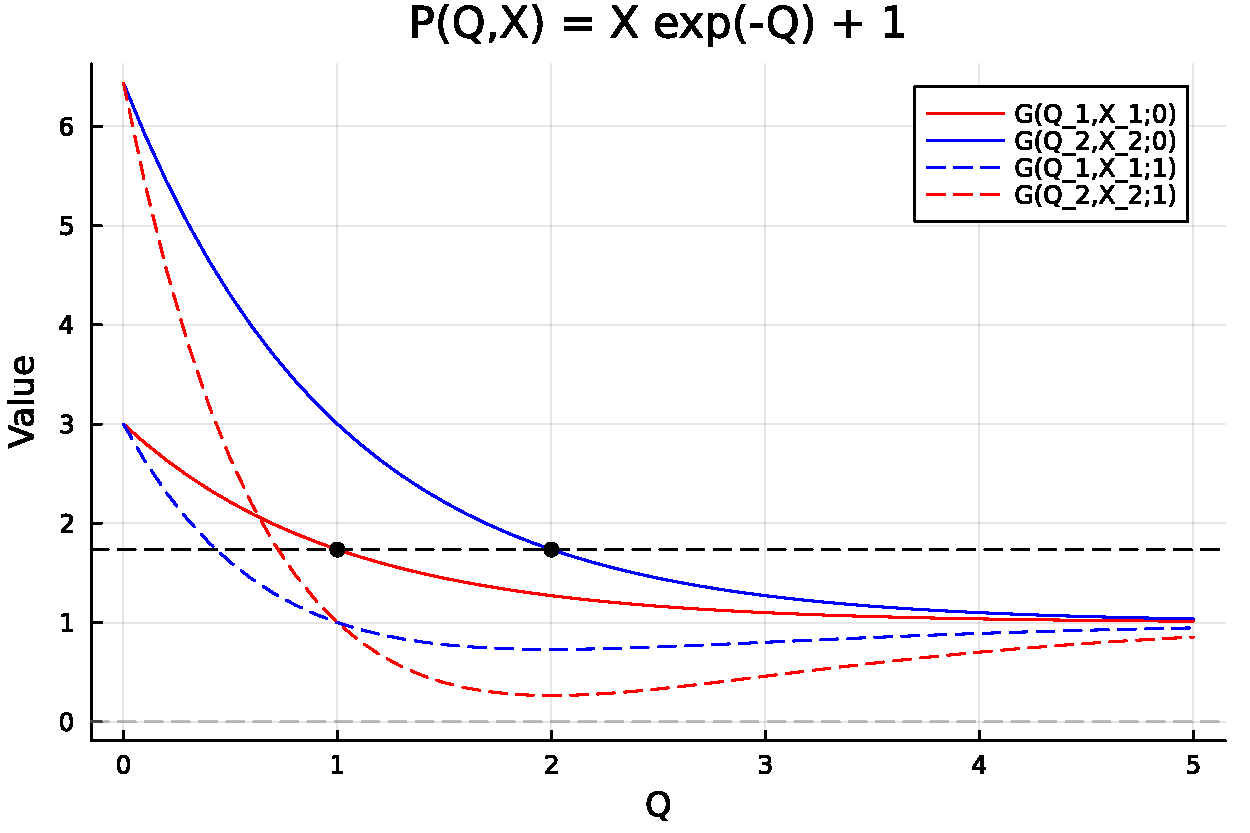
\includegraphics[width=0.8\textwidth]{../conduct_parameter/figuretable/plot_counter_example.pdf}
        \caption{The relationship between $MR(Q,X^{d};0)$ and $MR(Q,X^{d};1)$}
        \label{fig:counterxample_demand_curves}
    \end{center}
    The graph plots $MR(Q,X^{d};0)$ and $MR(Q,X^{d};1)$.
    The solid lines represent $MR(Q,X^{d};0)$ and the dashed lines represent $MR(Q,X^{d};1)$.
    The color corresponds to $(Q_1, X_1)$ and $(Q_2, X_2)$.
    $MR(Q,X^{d};0)$ takes the same value, but $MR(Q,X^{d};1)$ takes different values under $(Q_1, X_1)$ and $(Q_2, X_2)$.
    \end{figure}
\end{example}

Now, we show that there is an inverse demand function not satisfying \eqref{eq:identification_separable}, which does not satisfy the necessary condition for the existence of $T$.
Thus, we have shown that the inverse demand function \eqref{eq:identification_separable} cannot be the necessary condition for that $T$ does not exist.
This also implies that we can find an inverse demand function where observable equivalence is violated for any $Q$ and $X^{d}$.



\begin{remark}
There are several additional concerns about Lau's argument.
\begin{itemize}
    \item The transformation $T$ is defined as two-variables function, although Lemma \ref{lemma_1_GU} requires a function of one variable.
    Additionally, the two variables $P(Q^e, X^{d}) + \theta \frac{\partial P}{\partial Q}(Q^e, X^{d}) Q^e$ and $Q^e$ are regarded as independent variables.
    However, $Q^e$ is a function of $X^{d}$ and $X^{s}$ and both variables include $Q^e$.
    Therefore, the two variables cannot be independent.
    \item Note that \eqref{eq:singular_equation} holds for any quantity because Lau tries to find an inverse demand function that makes $T$ singular globally.
    In other words, an inverse demand function that violates observable equivalence for any $Q$ and $X^{d}$.
    However, this is much stronger than non-identification requires. If there exists an $X^{d}$ and $X^{s}$, and thus an equilibrium quantity $Q^e$, such that \eqref{eq:singular_equation} holds, then observable equivalence is violated at that point, which is sufficient to show non-identification.
\end{itemize}
\qed
\end{remark}



\subsection{Case 2: The demand shifter is a vector}
Suppose that the inverse demand function satisfies the transformation given by \eqref{eq:transformation_T_demand_la}.
When $X^{d}$ is a vector, \eqref{eq:transform_demand} can be written as
\begin{align}
    (1 -  \lambda(X^{d}, X^{s}))\frac{\partial P}{\partial X^{d}_{i}}(Q^e, X^{d}) = (  \lambda(X^{d}, X^{s})\theta  - \theta^*)\frac{\partial^2 P}{\partial X^{d}_{i}\partial Q}(Q^e, X^{d})Q^e.
\end{align}
By taking the ratio between $i$ and $j$, $(1 - \lambda(X^{d}, X^{s}))$ and  $(\theta\lambda(X^{d}, X^{s}) - \theta^{*})$ are canceled out, and hence we have
\begin{align}
    \frac{\frac{\partial P}{\partial X^{d}_{i}}(Q, X^{d})}{\frac{\partial P}{\partial X^{d}_{j}}(Q, X^{d})} & = \frac{ \frac{\partial^2 P}{\partial X^{d}_{i} \partial Q}(Q, X^{d})}{\frac{\partial^2 P}{\partial X^{d}_{j} \partial Q}(Q, X^{d})}\\
    \frac{\frac{\partial^2 P}{\partial X^{d}_{i} \partial Q}(Q, X^{d})}{\frac{\partial P}{\partial X^{d}_{i}}(Q, X^{d})}  & = \frac{\frac{\partial^2 P}{\partial X^{d}_{j} \partial Q}(Q, X^{d})}{\frac{\partial P}{\partial X^{d}_{j}}(Q, X^{d})}\\ 
    \frac{\partial }{\partial Q} \log\left( \frac{\partial P}{\partial X^{d}_{i}}(Q, X^{d})\right) &= \frac{\partial }{\partial Q} \log\left( \frac{\partial P}{\partial X^{d}_{j}}(Q, X^{d})\right)\\
    0& = \frac{\partial}{\partial Q}\log\left(\frac{\frac{\partial P}{\partial X^{d}_{i}}(Q, X^{d})}{\frac{\partial P}{\partial X^{d}_{j}}(Q, X^{d})}\right)
\end{align}
Note that we can exchange the order of partial derivative due to Young's theorem as $P$ is twice continuously differentiable.

Then, by the chain rule, we have
\begin{align}
    0 & = \left(\frac{\frac{\partial P}{\partial X^{d}_{i}}(Q, X^{d})}{\frac{\partial P}{\partial X^{d}_{j}}(Q, X^{d})}\right)^{-1} \frac{\partial}{\partial Q} \left(\frac{\frac{\partial P}{\partial X^{d}_{i}}(Q, X^{d})}{\frac{\partial P}{\partial X^{d}_{j}}(Q, X^{d})}\right).
    \label{eq:derivative_separable}
\end{align}

Because $X^{d}$ is defined as a vector of demand shifters that affect the inverse demand function, it is natural to think that $\partial P/\partial X^{d}_{i} \ne 0$ for all $i$.
Therefore, we should have
\begin{align}
    \frac{\frac{\partial P}{\partial X^{d}_{i}}(Q, X^{d})}{\frac{\partial P}{\partial X^{d}_{j}}(Q, X^{d})} \ne 0.
\end{align}
Therefore, the denominator in \eqref{eq:derivative_separable} is nonzero, which implies that the derivative with respect to $Q$ is zero;
\begin{align}
    \frac{\partial}{\partial Q} \left(\frac{\frac{\partial P}{\partial X^{d}_{i}}(Q, X^{d})}{\frac{\partial P}{\partial X^{d}_{j}}(Q, X^{d})}\right) = 0.
\end{align}
This is equivalent to the weak separability in \citet{goldmanNote1964}, and hence we can apply Theorem \ref{thorem_2_GU} to conclude that when $X^{d}$ is a vector, non-identification implies that the inverse demand function is a separable function.



\subsection{The summary of the argument for the necessity}
So far, we have shown two things.
\begin{itemize}
    \item When the demand shifter is a scalar, while Lau states that the conduct parameter cannot be identified except for the case where the inverse demand function satisfies \eqref{eq:identification_separable}, our argument shows there could be an inverse demand function that does not satisfy \eqref{eq:identification_separable} but observable equivalence is violated for any $Q$ and $X^{d}$.
    \item When the demand shifter is a vector, non-identification implies that the inverse demand function is a separable function.
\end{itemize}
At least for the case where the demand shifter is a scalar, our argument points out that Lau's argument is not correct.



\section{Sufficiency Proof in Lau(1982)}\label{sec:proof_lau_sufficiency}
Now, we show that when the inverse demand function is separable, we can find distinct sets of the conduct parameter and the marginal cost function that lead to observable equivalent equilibrium.
When the true inverse demand function satisfies \eqref{eq:identification_separable}, non-identification cannot hold.
Thus, the conduct parameter and the marginal cost function can be identified.

Assume that $(\theta, MC)$ is a true conduct parameter and marginal cost function and the inverse demand function is a separable $P = P(Q, r(X^{d}))$ but not satisfying  \eqref{eq:identification_separable}.
Pick up an alternative conduct parameter value $\theta^{*}$.
Suppose that there is a transformation $T$ such that
\begin{align}
    P(Q, r(X^d)) + \theta^{*}\frac{\partial P}{\partial Q}(Q, r(X^d)) Q 
    &= T\left(P(Q, r(X^d)) + \theta \frac{\partial P}{\partial Q}(Q, r(X^d)) Q, Q\right) \label{eq:sufficiency_transform_p}
\end{align}
for all $Q, X^d$.
While $X^{d}$ be a vector, \eqref{eq:sufficiency_transform_p} corresponds to the case $X^{d}$ is a scalar.
Therefore, we cannot identify the conduct parameter except when the separable satisfies \eqref{eq:identification_separable}.


Note that non-identification and the existence of $T$ are equivalent.
In other words, given $(\theta, MC)$ and $\theta^{*}$, $T$ can generate an observable equivalent equilibrium.
Under the true component $(\theta, MC)$, we can obtain the equilibrium quantity $Q^{e}$.
This quantity should solve the first-order condition 
\begin{align}
    P(Q^e, X^d) + \theta \frac{\partial P}{\partial Q}(Q^e, X^d) Q^e = MC(Q^e, X^{s}).
\end{align}
Then, by applying $T$, we have
\begin{align}
    P(Q^e, X^d) + \theta^{*} \frac{\partial P}{\partial Q}(Q^e, X^d) Q^e 
    & = T\left(P(Q^e, X^d) + \theta \frac{\partial P}{\partial Q}(Q^e, X^d) Q^e, Q^e\right) \\
    &= T( MC(Q^e, X^{s}), Q^e).
\end{align}
Define $MC^{*}(Q, X^{s}) \equiv T(MC(Q, X^{s}), Q)$.
Then, the above relationship implies that $Q^{e}$ also solves the first-order condition under $(\theta^{*}, MC^{*})$;
\begin{align}
    P(Q^e, X^d) + \theta^{*} \frac{\partial P}{\partial Q}(Q^e, X^d) Q^e = MC^{*}(Q^e, X^{s}).
\end{align}
Therefore, two distinct pairs of the conduct parameter and the marginal cost lead to the same equilibrium quantity.


This implies that when separable inverse demand function guarantees that there is a transformation $T$ such that \eqref{eq:sufficiency_transform_p} holds for any $Q$ and $X^{d}$, we can construct a pair of the conduct parameter and the marginal cost function that leads to the same equilibrium quantity.
However, this is not the case.
Note that the inverse demand function in Example \ref{counter_example_demand_curves} is separable.
But, we have seen that we cannot have a transformation $T$ under the inverse demand function in the example.
Therefore, Lau's argument for sufficiency is also not correct.














\section{Correct proof}



Suppose that there exists a transformation $T$ such that
\begin{align}
    P(Q, r(X^d)) + \theta^{*}\frac{\partial P}{\partial Q}(Q, r(X^d)) Q 
    &= T\left(P(Q, r(X^d)) + \theta \frac{\partial P}{\partial Q}(Q, r(X^d)) Q, Q\right)
\end{align}
for all $Q, X^d$.


Then, we have
\begin{align}
    \frac{MR(Q_1, X_1^d; \theta^{*})}{MR(Q_1, X_1^d; \theta)} = \frac{MR(Q_2, X_2^d; \theta^{*})}{MR(Q_2, X_2^d; \theta)}
\end{align}
for any $Q_1, Q_2, X_1^d, X_2^d$.
This also implies that the ratio 
\begin{align}
    \frac{MR(Q, X^d; \theta^{*})}{MR(Q, X^d; \theta)} = \frac{P(Q, X^d) + \theta^{*}\frac{\partial P}{\partial Q}(Q, X^d) Q}{P(Q, X^d) + \theta \frac{\partial P}{\partial Q}(Q, X^d) Q}
\end{align}
is a constant for any $Q$ and $X^d$.
Divide the numerator and the denominator by $P$, we have
\begin{align}
    \frac{1 + \theta^{*}\frac{\partial P}{\partial Q}(Q, X^d) \frac{Q}{P(Q, X^d)}}{1 + \theta \frac{\partial P}{\partial Q}(Q, X^d) \frac{Q}{P(Q, X^d)}} = \frac{1 - \theta^{*}\varepsilon(X^d)}{1 - \theta \varepsilon(X^d)}
\end{align}
where $\varepsilon(X^d)$ is the price elasticity of demand and is a function of $X^d$.
When this is a constant for any $Q$ and $X^d$, we should have that the elasticity is also a constant;
\begin{align}
    \frac{\partial \log P(Q, X^d)}{\partial \log Q}  = k
\end{align}
for some constant $k$.
Therefore, the inverse demand function should be a constant elasticity function.


This is an differential equation.
To solve this, assume that $P(Q, X^d) = Q^{k}r(X^{d})$.
Then, we have
\begin{align}
    \frac{\partial \log P(Q, X^d)}{\partial \log Q}  = k.
\end{align}
This is a separable differential equation.











\iffalse



\subsubsection*{A corrected argument 1}
Now, we present a corrected argument.
From \eqref{eq:derivative_q_x_d} and \eqref{eq:derivative_q_x_s}, we have
\begin{align}
    &\frac{\partial P}{\partial X^{d}_{i}}(Q^e, X^{d}) + \theta^{*}\frac{\partial^2 P}{\partial X^{d}_{i}\partial Q}(Q^e, X^{d})Q^e \\
    &\hspace{2cm} = \lambda(X^{d}, X^{s})\left[\frac{\partial P}{\partial X^{d}_{i}} (Q^e, X^{d})+ \theta \frac{\partial^2 P}{\partial X^{d}_{i}\partial Q}(Q^e, X^{d})Q^e\right],\label{eq:transform_demand}
\end{align}
and
\begin{align}
    \frac{\partial MC^{*}}{\partial X^{s}_{i}}(Q^e, X^{s}) & = \lambda(X^{d}, X^{s})\frac{\partial MC}{\partial X^{s}_{i}}(Q^e, X^{s}),\label{eq:transform_mc}
\end{align}
where $\lambda(X^{d}, X^{s})$ is defined as
\begin{align}
    \lambda( X^{d}, X^{s}) \equiv \frac{(1+\theta^{*})\frac{\partial P}{\partial Q}(Q^e, X^{d}) + \theta^{*}\frac{\partial^2 P}{\partial Q^2}(Q^e, X^{d})Q^e - \frac{\partial MC^{*}}{\partial Q}(Q^e, X^{s})}{(1+\theta)\frac{\partial P}{\partial Q}(Q^e, X^{d}) + \theta\frac{\partial^2 P}{\partial Q^2}(Q^e, X^{d})Q^e - \frac{\partial MC}{\partial Q}(Q^e, X^{s})}.\label{eq:lambda_q_x}
\end{align}
In our definition, $\lambda$ is a function of $X^{d}$ and $X^{s}$ to express that $Q^e$ is a function of $X^{d}$ and $X^{s}$.
This is well-defined because the denominators in \eqref{eq:derivative_q_x_d} and \eqref{eq:derivative_q_x_s} are assumed to be nonzero.
By applying Lemma \ref{lemma_1_GU} to \eqref{eq:transform_demand} and \eqref{eq:transform_mc}, there is a transformation $T$ such that
\begin{align}
    P(Q^e, X^{d}) + \theta^{*} \frac{\partial P}{\partial Q}(Q^e, X^{d}) Q^e & = T\left(P(Q^e, X^{d}) + \theta \frac{\partial P}{\partial Q}(Q^e, X^{d}) Q^e\right) \label{eq:transformation_T_demand}
\end{align}
and
\begin{align}
    MC^{*}(Q^e, X^{s}) = T(MC(Q^e, X^{s})), \label{eq:transformation_T_mc}
\end{align}
for any $X^{d}$, $X^{s}$ and $Q^e = h(X^{d}, X^{s})$.
Here, as Lemma \ref{lemma_1_GU} requires $T$ to be a function of one variable, we express as a one-variable function.
Therefore, the first-order condition under the true component $(\theta, MC)$ can be transformed into the first-order condition under $(\theta^*, MC^*)$ through $T$ while keeping the equilibrium quantity the same.
Additionally, we use both \eqref{eq:derivative_q_x_d} and \eqref{eq:derivative_q_x_s} to derive \eqref{eq:transformation_T_demand} and \eqref{eq:transformation_T_mc}.

















\subsubsection{The cases where observable equivalence does not hold}



% OEとダイレクトにつなげた議論

In the following, we proceed to the argument which has the same implication with Lau but is based on observable equivalence.
First, suppose that
\begin{align}
    \frac{\partial MC}{\partial X_i^{s}}(Q, X^{s}) = 0, \frac{\partial MC^{*}}{\partial X_i^{s}}(Q, X^{s}) \ne 0.
\end{align}
Then, the right-hand side of \eqref{eq:transform_mc} is zero, although its left-hand side is nonzero.
Thus, \eqref{eq:transform_mc} cannot hold.
This situation also implies that the observable equivalence does not hols because $\frac{\partial h^{*}}{\partial X^{s}_{i}}  \ne \frac{\partial h}{\partial X^{s}_{i}}$ in \eqref{eq:derivative_q_x_s}.
Fortunately, Lau assumes that $X^{s}$ is the vector of cost shifter that affects the marginal cost function, and hence, it is natural to assume that for any marginal cost function $MC$, 
\begin{align}
    \frac{\partial MC}{\partial X_i^{s}}(Q, X^{s}) \ne 0.
\end{align}


% There may not be a transformation for the demand function

In contrast, we need more careful consideration for \eqref{eq:transform_demand}.
Suppose that the inverse demand function $P$ satisfies
\begin{align}
    \frac{\partial P}{\partial X^{d}_{i}}(Q, X^{d}) + \theta \frac{\partial^2 P}{\partial X^{d}_{i}\partial Q}(Q, X^{d})Q = 0,\\
    \frac{\partial P}{\partial X^{d}_{i}}(Q, X^{d}) + \theta^{*} \frac{\partial^2 P}{\partial X^{d}_{i}\partial Q}(Q, X^{d})Q \ne 0. 
\end{align}
This situation violates the observable equivalence because $\frac{\partial h^{*}}{\partial X^{d}_{i}}  \ne \frac{\partial h}{\partial X^{d}_{i}} =0$.
Note that the first equation is a partial differential equation.


% Vector case and scalar case
\subsubsection{The cases where observable equivalence hold}
Now, we exclude the case where observable equivalence does not hold.
We want to find the inverse demand function that non-identification implies.

\subsubsection*{Case: $X^{d}$ is a scalar}
When $X^{d}$ is a scalar,  \eqref{eq:transform_demand} becomes
\begin{align}
    &\frac{\partial P}{\partial X^{d}}(Q^e, X^{d}) + \theta^{*}\frac{\partial^2 P}{\partial X^{d}\partial Q}(Q^e, X^{d})Q^e \\
    &\hspace{2cm} = \lambda(X^{d}, X^{s})\left[\frac{\partial P}{\partial X^{d}} (Q^e, X^{d})+ \theta \frac{\partial^2 P}{\partial X^{d}\partial Q}(Q^e, X^{d})Q^e\right].
\end{align}
In this case, Lau does not characterize the inverse demand function where the above equation holds.
Thus, Lau concludes that the conduct parameter and the marginal cost function cannot be identified except \eqref{eq:identification_separable}.
\textcolor{red}{(Q: is there a demand function that non-identification implies when $X^{d}$ is a scalar?)}






























Because \eqref{eq:sufficiency_transform_p} is equivalent to non-identification, an important question is whether we always have a transformation $T$  when the demand function is separable.




















For any $\theta$, we have
\begin{align}
    \frac{\partial P}{\partial X^{d}}(Q, X^{d}) + \theta \frac{\partial^2 P}{\partial X^{d}\partial Q}(Q, X^{d})Q  = \exp(-Q) (1 - \theta Q).
\end{align}
Therefore, when $(1 - \theta Q^e) = 0$, we have that $\frac{\partial h}{\partial X_{i}^d} = 0$ and $\frac{\partial h^{*}}{\partial X^d} \ne 0$.
While \eqref{eq:identification_separable} requires that $\frac{\partial h}{\partial X_{i}^d} =0$ holds for any $Q$ and $X^{d}$, the above inverse demand requires $\frac{\partial h}{\partial X_{i}^d}  = 0$ only at $Q^e = \frac{1}{\theta}$.

The inverse demand is decreasing in $Q$.
For example, when the true marginal function is a linear function such that $MC(Q, X^{s}) = \beta_1 Q + \beta_1X^s$, we can easily find the unique equilibrium.




\begin{figure}[th]
    \begin{center}
        \includegraphics[width=0.8\textwidth]{../conduct_parameter/figuretable/plot_counter_example_specific_function.pdf}
        \caption{The relationship between $MR(Q,X^{d};0)$ and $MR(Q,X^{d};1)$}
        \label{fig:counterxample_demand_curves_specific_function}
    \end{center}
    The graph plots $MR(Q,X^{d};0)$ and $MR(Q,X^{d};1)$.
    The solid lines represent $MR(Q,X^{d};0)$ and the dashed lines represent $MR(Q,X^{d};1)$.
    The color corresponds to $(Q_1, X_1)$ and $(Q_2, X_2)$.
    $MR(Q,X^{d};0)$ takes the same value, but $MR(Q,X^{d};1)$ takes different values under $(Q_1, X_1)$ and $(Q_2, X_2)$.
\end{figure}
    





























\fi

\section{Discussion}

\subsection{Relation to the recent literature on distinguishing firm conduct}

The sufficiency of separability implies that if the conduct parameter and marginal cost are simultaneously identified, the demand function is non-separable or satisfies the specific separable function form.
However, the recent literature uses a broader variation in markets for the identification of conduct beyond demand shifters and rotators.
For example, in the differentiated product environment, \citet{berry2014identification} demonstrate that the change in marginal cost or the market size is useful, and hence demand rotation instruments are not necessary to identify conduct.

Of course, homogeneous product settings are more restricted than differentiated product settings.
Even so, Lau's proof of sufficiency does not show that unless a separable demand satisfies  \eqref{eq:identification_separable}, there always exist two distinct pairs of conduct parameter and marginal cost.
Therefore, there could be a separable function except \eqref{eq:identification_separable} that can achieve identification based on other variations in markets.



\section{Conclusion}

We present a counterexample to \citet{lau1982identifying}'s identification result, showing that a separable demand function outside his specified form can still achieve identification of both the conduct parameter and the marginal cost. This finding, supported by theoretical analysis and numerical simulations, challenges existing assumptions for identifying the conduct parameter beyond the linear specification of demand and marginal cost functions.

\paragraph{Acknowledgments}
We thank Jeremy Fox and an anonymous referee for their invaluable comments and Kaede Hanazawa for his excellent research assistance.
This work was supported by JST ERATO Grant Number JPMJER2301, Japan.  


\newpage
\bibliographystyle{aer}
\bibliography{conduct_parameter.bib}





\appendix


\section{Omitted proofs and calculations}\label{app:ommitted_proof}

\subsection{Solving the partial differential equation when the transformation is singular}
Recall that when the transformation is singular, we have
\begin{align}
    \frac{\partial P}{\partial X^{d}_{i}}(Q, X^{d}) + \theta \frac{\partial^2 P}{\partial X^{d}_{i}\partial Q}(Q, X^{d})Q = 0.
\end{align}
This is a partial differential equation of $P(Q, X^{d})$.
To solve the equation, assume that the inverse demand function is a separable function such that 
\[P(Q, X^{d}) = g(Q)h(X^{d}) + s(Q).\]
By substituting the separable function into the differential equation, we have 
\begin{align}
   0 & =  g(Q) h_i(X^{d}) + \theta g'(Q)h_i(X^{d}) Q\\
   & = h_i(X^{d})( g(Q) + \theta g'(Q)Q).
\end{align}
When $h_i(X^{d}) = 0$, the inverse demand does not react to the change in $X^{d}$, which is unrealistic in this model.
Therefore, we should assume that $h_i(X^{d}) \ne 0$, and hence we have 
\[g(Q) + \thetag'(Q)Q = 0.\]
This equation is an ordinary differential equation of $Q$ of $g(Q)$.
This can be written as
\begin{align}
    \frac{g'(Q)}{g(Q)} &= -\frac{1}{\theta} \frac{1}{Q}
\end{align}
Because the left-hand side is the derivative of $\log g(Q)$ and the right-hand side is also a derivative of $\log Q$, we have
\begin{align}
        \frac{d}{dQ} \log g(Q) &= -\frac{1}{\theta} \frac{d}{dQ} \log Q.
\end{align}
By integrating this over the domain of $Q$, we have
\begin{align}
    \int_{0}^\infty \frac{d}{dQ} \log g(Q) dQ &= -\frac{1}{\theta} \int_{0}^\infty  \frac{d}{dQ} \log Q dQ \\
    \log g(Q) &= -\frac{1}{\theta} \log Q + C\\
    g(Q) &= C Q^{-\frac{1}{\theta}},
\end{align}
where $C$ is the constant of integration.
Substituting this into $f$, we have 
\begin{align}
    P(Q, X^{d}) = C Q^{-\frac{1}{\theta}} h(X^{d}) + s(Q).
\end{align}
Define $r(X^{d}) = Ch(X^{d})$, and then we have
\begin{align}
    P(Q, X^{d}) &= Q^{-\frac{1}{\theta}} r(X^{d}) + s(Q),
\end{align}
which is the same with \eqref{eq:identification_separable}.


\subsubsection{Checking whether observable equivalence is violated}
When the inverse demand function satisfies \eqref{eq:identification_separable}, we have $\frac{\partial h}{\partial X^{d}_{i}}(X^{d}, X^{s}) = 0$.
Now, we check whether $\frac{\partial h^{*}}{\partial X_{i}^{d}} \ne 0$ for an alternative conduct parameter $\theta^{*} \ne \theta$.
In this case, the observable equivalence is violated for any $X^{d}$ and $X^{s}$.

By substituting the inverse demand function \eqref{eq:identification_separable} into $\frac{\partial h^{*}}{\partial X_{i}^d}$, we have
\begin{align}
    \frac{\partial h^{*}}{\partial X_{i}^d} = \frac{\partial P}{\partial X^{d}_{i}} + \theta^{*} \frac{\partial^2 P}{\partial X^{d}_{i}\partial Q}Q  &= Q^{-1/\theta} r_i(X^d) - \frac{\theta^{*}}{\theta} Q^{-1/\theta-1} r_i(X^d) Q\\
    &= Q^{-1/\theta} r_i(X^d) \left(1 - \frac{\theta^{*}}{\theta} \right).
\end{align}
This becomes zero if and only if $\theta= \theta^{*}$.
Hence for any $\theta^{*} \ne \theta$, $\frac{\partial h^{*}}{\partial X_{i}^{d}} \ne 0$ holds when the inverse demand satisfies \eqref{eq:identification_separable}.
That is, under the specific inverse demand \eqref{eq:identification_separable}, we always have 
\begin{align}
    \frac{\partial h^{*}}{\partial X^{d}_{i}}(X^{d}, X^{s}) \ne \frac{\partial h}{\partial X^{d}_{i}}(X^{d}, X^{s}) = 0.
\end{align}


\subsubsection{Checking whether the equilibrium exists}
We still need an additional step because there could be the possibility that there is no equilibrium under the separable function.
In other words, we cannot solve the first-order condition under the true $(\theta, MC)$.
Substitute the separable inverse demand function \eqref{eq:identification_separable} into \eqref{eq:foc_alpha}, obtaining
\begin{align}
    P(Q, X^{d}) + \theta \frac{\partial P}{\partial X_i^{d}} (Q, X^{d}) Q & =  Q^{-\frac{1}{\theta}} r(X^{d}) + s(Q) + \theta \left(-\frac{1}{\theta}\right) \left[  Q^{-\frac{1}{\theta} -1} r(X^{d}) + s'(Q)\right]Q\\
    & = s(Q) - s'(Q)Q.
\end{align}
The first-order condition implies that
\begin{align}
    s(Q) - s'(Q)Q = MC(Q, X^{s}).
\end{align}
The quantity that solves the equation becomes the equilibrium quantity.
The equation is similar to the first-order condition of the monopolistic firm without demand shifters.
Thus, $s(Q)$ also needs some conditions to guarantee the uniqueness of the equilibrium.
This implies that the equilibrium quantity does not depend on $X^{d}$ and only depends on $X^{s}$, which is consistent with $\frac{\partial h}{\partial X^{d}_{i}}(X^{d}, X^{s}) = 0$.










\section{A counterexample}

We show that the conduct parameter is identified when the inverse demand function is separable. 
Consider the following inverse demand function and marginal cost function:
\begin{align}
    P & = \exp(\varepsilon_{d}) Q^{\alpha_0} X_{d1}^{\alpha_1}X_{d2}^{\alpha_2}\label{eq:counter_demand}\\
    MC & = \exp(\varepsilon_{s})Q^{\beta_0} X_{s1}^{\beta_1} X_{s2}^{\beta_2}.\label{eq:counter_mc}
\end{align}
Assume that $\alpha_0 <0$.
The above model does not have an intercept in both the demand function and the marginal cost function. 

The inverse demand function is separable because
\begin{align}
    \frac{\partial }{\partial Q} \left(\frac{\partial P/\partial X_{d1}}{\partial P/\partial X_{d2}} \right) = \frac{\partial }{\partial Q} \left(\frac{\alpha_{1}\exp(\varepsilon_{d}) Q^{-\alpha_0} X_{d1}^{\alpha_1-1}X_{d2}^{\alpha_2}}{\alpha_2\exp(\varepsilon_{d}) Q^{-\alpha_0} X_{d1}^{\alpha_1}X_{d2}^{\alpha_2-1}} \right) =  \frac{\partial }{\partial Q}\left(\frac{\alpha_1}{\alpha_2} \frac{X_{d2}}{X_{d1}} \right)=0.
\end{align}
Thus Theorem \ref{theorem_lau} implies that the conduct parameter cannot be identified.
By taking logarithm to \eqref{eq:counter_demand}, we have a log-linear demand equation such that 
\begin{align}
    \log P = \alpha_0 \log Q + \alpha_1 \log X_{d1}  + \alpha_2 \log X_{d2} + \varepsilon_{d}.\label{eq:counter_demand_equation}
\end{align}
From the first-order condition, 
\begin{align}
    MC = Q^{\beta_0} X_{s1}^{\beta_1}X_{s2}^{\beta_2}\exp(\varepsilon_{s}) & = P + \theta (\alpha_0 \exp(\varepsilon_{d})Q^{\alpha_0-1}X_{d1}^{\alpha_1}X_{d2}^{\alpha_2}) Q\\
    & = P + \theta \alpha_0 P\\
    &= (1 + \theta\alpha_0) P.
\end{align}
By taking a logarithm, we obtain a log-linear supply equation,
\begin{align}
    \log P = - \log(1 + \theta\alpha_0) + \beta_0 \log Q + \beta_1 \log X_{s1}+\beta_2 \log X_{s2} + \varepsilon_{s}.\label{eq:counter_supply_equation}
\end{align}
By solving \eqref{eq:counter_demand_equation} and \eqref{eq:counter_supply_equation}, the equilibrium quantity $Q$ is obtained as
\begin{align}
    \log Q = \frac{\beta_1 \log X_{s1}+\beta_2 \log X_{s2} - \log(1 + \theta\alpha_0)+ \varepsilon_{s} - \alpha_1 \log X_{d1}  - \alpha_2 \log X_{d2} - \varepsilon_{d} }{\alpha_0 - \beta_0}.
\end{align}

Note that the demand parameters can be identified when $X^s$ is a vector of exclusive demand instruments.
Thus we can assume that $\alpha_0, \alpha_1$, and $\alpha_2$ is known.  

Then it is easy to see that $- \log(1 + \theta\alpha_0), \beta_0$, and $\beta_1$ are identified with a vector of exclusive supply instrument $X^d$.
Let $\gamma = - \log(1 + \theta\alpha_0)$, then $\theta = (\exp(-\gamma) - 1)/\alpha_0$.
Because $\alpha_0$ is identified, the parameter $\theta$ is also identified, which contradicts Theorem \ref{theorem_lau}.
\begin{remark}
    The above inverse demand function has a constant-elasticity property. 
    Note that $\alpha_0 \ne \frac{1}{\theta}$ holds.
    Thus it is not the separable function that allows identification in Theorem \ref{theorem_lau}.
    However, \citet{lau1982identifying} states that under this functional form, the conduct parameter cannot be identified in his comment (2) in p 98.
\end{remark}

\begin{remark}
    When the demand equation and the marginal cost equation have an intercept, the identification is impossible because the constant term in \eqref{eq:counter_supply_equation} becomes $-\log(1+\theta \alpha_0) + \beta$ and $\beta$ and $\theta$ cannot be separately identified without additional variables such as demand rotation parameter.
\end{remark}



\section{Interpretation}


Let's return to the original idea in \citet{bresnahan1982oligopoly}.
He essentially considers the following model:
\begin{align}
    P & = \alpha_0 - \alpha_1 Q + \alpha_2 X^d + \varepsilon_d,\label{eq:bresnahan_demand} \\
    MC & = \beta_0 + \beta_1 Q + \beta_2 X^s + \varepsilon_s. \label{eq:bresnahan_marginal_cost}
\end{align}
Assume that $\alpha_1>0$ and $\beta_1 >0$.
The marginal revenue under $\theta$ is
\begin{align}
    MR = \alpha_0 - \alpha_1(1 + \theta) Q + \alpha_2 X^d + \varepsilon_d. \label{eq:bresnahan_marginal_revenue}
\end{align}
Note that when $\theta = 1$, the slope of the marginal revenue is twice as steep as the demand function under a linear demand model.

The first-order condition implies that the intersection between the marginal revenue \eqref{eq:bresnahan_marginal_revenue} and the marginal cost \eqref{eq:bresnahan_marginal_cost} determines the equilibrium quantity.
The other way to get the equilibrium quantity is to use the demand function and the supply function.
Based on the first-order condition, the supply relation can be computed as
\begin{align}
    P & = \beta_0 + (\beta_1 + \theta\alpha_1) Q  + \beta_2 X^s + \varepsilon_s.\label{eq:bresnahan_supply}
\end{align}
The intersection of \eqref{eq:bresnahan_demand} and \eqref{eq:bresnahan_supply} derives the equilibrium price and the equilibrium quantity.
The equilibrium quantity is given by
\begin{align}
    Q = \frac{\alpha_0 + \alpha_2 X^d - \beta_0 - \beta_2 X^s + \varepsilon_d - \varepsilon_s}{\alpha_1(1 + \theta) +  \beta_1}.
\end{align}

For a true marginal cost parameter $\beta$ and the conduct parameter $\theta$, consider the marginal cost parameter of the alternative model given by
\begin{align}
    \beta_0^{*} = \beta_0, \quad \beta_1^{*} = \beta_1 + \alpha_1(\theta - \theta^{*}), \quad \beta_2^{*} = \beta_2.
\end{align}
Thus, the marginal cost under the alternative model is different from the true model only in the coefficient of $Q$.
In this case the model with $(\theta, \beta)$ is observationally equivalent to the model with $(\theta^{*}, \beta^{*})$.


In \citet{bresnahan1982oligopoly}, he considers perfect competition ($\theta = 0$) and monopoly ($\theta = 1$).
Assume that the true model is the perfect competition, and then monopoly is the alternative model.
Then, the marginal cost parameter $\beta^{*}$ of the alternative model is given by
\begin{align}
    \beta_0^{*} = \beta_0, \quad \beta_1^{*} = \beta_1 - \alpha_1, \quad \beta_2^{*} = \beta_2.
\end{align}

In this example, the equilibrium quantity in the true model is given by
\begin{align}
    Q = \frac{\alpha_0 + \alpha_2 X^d - \beta_0 - \beta_2 X^s + \varepsilon_d - \varepsilon_s}{\alpha_1 + \beta_1}
\end{align}
The equilibrium quantity in the alternative model is given by
\begin{align}
    Q^{*} = \frac{\alpha_0 + \alpha_2 X^d - \beta_0^{*} - \beta_2^{*} X^s + \varepsilon_d - \varepsilon_s}{2\alpha_1 + \beta_1^{*}}.
\end{align}
Then, by the assumption on $\beta^{*}$, the equilibrium quantity is the same in both models ($Q = Q^{*}$) for any $X^d$ and $X^s$ because the denominator has the same value, and hence, the researcher cannot distinguish two models from the data.

Figure \ref{fig:bresnahan_non_identification} illustrates this situation.
$E_1$ is the observed equilibrium outcome, and both models rationalize the equilibrium.
Furthermore, the demand shift due to the increase of $X^d$ does not help identify the conduct, which equally increases $Q$ and $Q^{*}$, and $E_2$, the new equilibrium point, is still rationalized by both models.

We can also demonstrate that the conduct parameter cannot be identified in the supply relation \eqref{eq:bresnahan_supply}.
Let $\gamma = (\beta_1 + \theta \alpha_1)$.
Then, the parameter can be identified  in \eqref{eq:bresnahan_supply} are $\beta_0$,$\gamma$, and $\beta_2$, but we cannot identify $\theta$ as $\gamma$ in both models has the same value; 
\begin{align}
    \gamma &= \beta_1 + \theta \alpha_1 = \beta_1 = \beta_1 + \alpha_1 = \gamma^{*}.
\end{align}

\begin{figure}
    \begin{center}
        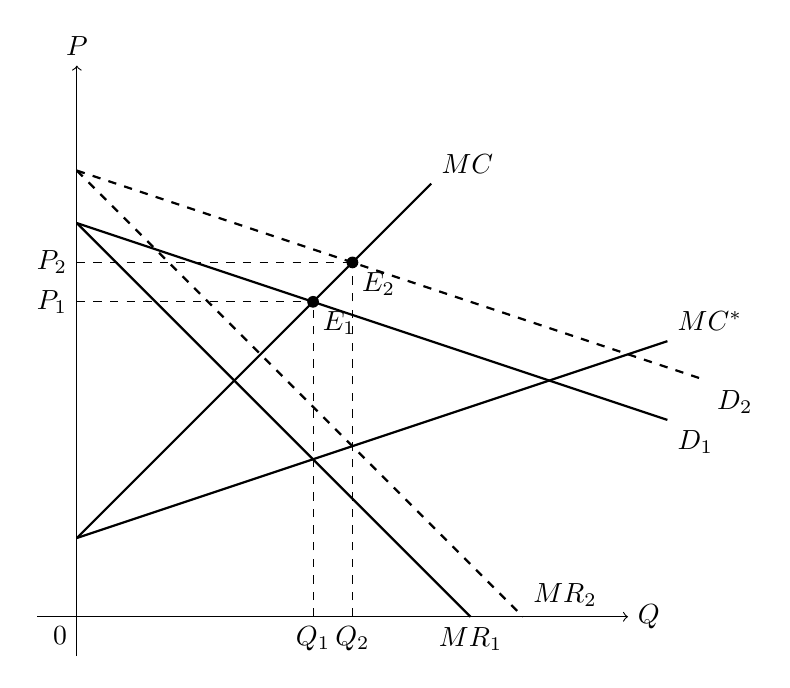
\begin{tikzpicture}
        % Axes
        \draw[->] (-0.5,0) -- (7,0) node[right] {$Q$}; % Horizontal axis
        \draw[->] (0,-0.5) -- (0,7) node[above] {$P$}; % Vertical axis
    
        % Demand Curve (D_1) - passes through (0,5), (3,4), and (7.5,2.5)
        \draw[thick] (0,5) -- (7.5,2.5) node[below right] {$D_1$};
    
        % Marginal Revenue (MR_1) - passes through (0,5), (3,2), and (5,0)
        \draw[thick] (0,5) -- (5,0) node[below] {$MR_1$};
    
        % Supply Curve under competition (S^c) - passes through (0,1), (3,4), and (4.5,5.5)
        \draw[thick] (0,1) -- (4.5,5.5) node[above right] {$MC$};
    
        % Supply Curve under monopoly (S^m) - passes through (0,1), (3,2), and (7.5,3.5)
        \draw[thick] (0,1) -- (7.5,3.5) node[above right] {$MC^{*}$};
    
        % Equilibrium point (E_1) - intersection of D_1 and S^c at (3,4)
        \node[circle, fill, inner sep=1.5pt] (E1) at (3,4) {};
        \node[below right] at (E1) {$E_1$};
    
    
        % Equilibrium point (E_2) - intersection of D_1 and S^c at (7/2,9/2)
        \node[circle, fill, inner sep=1.5pt] (E2) at (7/2,9/2) {};
        \node[below right] at (E2) {$E_2$};
    
        % Shifted Demand Curve (D_1 shifted)
        \draw[thick, dashed] (0,34/6) -- (8,3) node[below right] {$D_2$};
        
        % Shifted MR (MR_1 shifted)
        \draw[thick, dashed] (0,34/6) -- (34/6,0) node[above right] {$MR_2$};
        
        % Dashed lines for price and quantity
        \draw[dashed] (3,0) -- (3,4);
        \draw[dashed] (0,4) -- (3,4);
    
        \draw[dashed] (0,9/2) -- (7/2,9/2);
        \draw[dashed] (7/2,0) -- (7/2,9/2);
    
        % Additional labels
        \node[below left] at (0,0) {0};
        \node[left] at (0,4) {$P_1$};
        \node[below] at (3,0) {$Q_1$};
    
        \node[left] at (0,9/2) {$P_2$};
        \node[below] at (7/2,0) {$Q_2$};
    \end{tikzpicture}
    \end{center}
    \caption{The illustration of the non-identification result}
    \label{fig:bresnahan_non_identification}
    \vspace{2mm}
    \footnotesize
    Note: $MC$ is the marginal cost rationalized by the perfect competition, and $MC^{*}$ is the marginal cost rationalized by the perfect competition. $\beta_c = \beta_m + \alpha_1$ holds.
    The perfect competition and the monopoly rationalize the equilibrium point $E_1$. The shift in the demand does not help because the new equilibrium $E_2$ still are rationalized by both models.
\end{figure}


Now, let's investigate the same model with Lau's argument.
As Figure \ref{fig:bresnahan_non_identification} shows, the demand function and the marginal revenue with $\theta = 1$ have different slopes.
$MC$ and $MC^{*}$ are also different in the slope.

\begin{align}
    (1+\theta) \frac{\partial P}{\partial Q}(Q, X^d) + \theta \frac{\partial^2 P}{\partial Q^2}(Q, X^d) Q  - \frac{\partial MC}{\partial Q}(Q, X^s) = -\alpha_1(1 + \theta)   - \beta_1
\end{align}

Due to the assumption on the marginal cost parameter between $MC$ and $MC^{*}$,
\begin{align}
    \lambda(X^{d}, X^{s}) = \frac{-2\alpha_1  - \beta_1^{*}}{-\alpha_1  - \beta_1} =   \frac{-2\alpha_1  -\beta_1 + \alpha_1}{-\alpha_1  - \beta_1} = 1.
\end{align}

The numerator of \eqref{eq:derivative_q_x_d} is given by
\begin{align}
    \frac{\partial P}{\partial X^{d}}(Q, X^{d}) + \theta\frac{\partial^2 P}{\partial X^{d}\partial Q}(Q, X^{d})Q   = \alpha_2
\end{align}
and the numerator of \eqref{eq:derivative_q_x_s} is given by
\begin{align}
    \frac{\partial MC}{\partial X^{s}}(Q, X^{s}) = \beta_2.
\end{align}
Then, \eqref{eq:derivative_q_x_d} and \eqref{eq:derivative_q_x_s} are 
\begin{align}
    \frac{\partial h}{\partial X^{d}}(Q, X^{d}) = \frac{\partial h^{*}}{\partial X^{d}}(Q, X^{d})  = \frac{\alpha_2}{\alpha_1 + \beta_1},\\
    \frac{\partial h}{\partial X^{s}}(Q, X^{s}) = \frac{\partial h^{*}}{\partial X^{s}}(Q, X^{s})  =-\frac{\beta_2}{\alpha_1 + \beta_1}.
\end{align}
which implies that observable equivalence holds for any $X^d$ and $X^s$.


By applying Lemma \ref{lemma_1_GU}, we can say that there is a transformation $T$ such that
\begin{align}
    P(Q, X^d) + \frac{\partial P}{\partial Q}(Q, X^d) Q & = T(P(Q, X^d), Q)\\
    MC^{*}(Q, X^s) &= T(MC(Q, X^s), Q).
\end{align}
In this case, consider the following transformation:
\begin{align}
    T(x, Q) = x + \alpha_1(\theta - \theta^{*})Q.
\end{align}
Then, we have
\begin{align}
    T(MC(Q, X^s), Q) & =  \beta_0 + \beta_1 Q + \beta_2 X^s + \alpha_1(\theta - \theta^{*})Q\\
    & = \beta_0^{*} + \beta_1^{*} Q + \beta_2^{*} X^s\\
    & = MC^{*}(Q, X^s).
\end{align}
and
\begin{align}
    T\left(P(Q, X^d) + \theta \frac{\partial P}{\partial Q}(Q, X^d) Q, Q\right) & = P(Q, X^d) -\theta \alpha_1 Q +  \alpha_1(\theta - \theta^{*})Q\\ 
    & = P(Q, X^d) - \theta^{*} \alpha_1 Q  \\
    & = P(Q, X^d) + \theta^{*} \frac{\partial P}{\partial Q}(Q, X^d) Q.
\end{align}
The transformation $T$ also properly transforms the first-order condition;
\begin{align}
    &T\left(P(Q, X^d) + \frac{\partial P}{\partial Q}(Q, X^d) Q, Q\right) - T(MC(Q, X^s), Q)\\
    &= P(Q, X^d) + \theta^{*} \frac{\partial P}{\partial Q}(Q, X^d) Q - MC^{*}(Q, X^s).
\end{align}
Thus, the transformation generates the observable equivalent equilibrium.






As we have seen, the existence of the transformation $T$ implies for different $Q$ and $X^d$ and $X^s$,
\begin{align}
    P(Q_1, X^{d}_1) = P(Q_2, X^{d}_2) \Longrightarrow P(Q_1, X^{d}_1) + \frac{\partial P}{\partial Q}(Q_1, X^{d}_1) Q_1 = P(Q_2, X^{d}_2) + \frac{\partial P}{\partial Q}(Q_2, X^{d}_2) Q_2
\end{align}
and
\begin{align}
    MC(Q_1, X^{s}_1) = MC(Q_2, X^{s}_2) \Longrightarrow MC^*(Q_1, X^{s}_1) = MC^*(Q_2, X^{s}_2).
\end{align}
However, this cannot holds in this setting.

Figure \ref{fig:bresnahan_non_transformation} illustrates this situation.
$E_1$ is the equilibrium point with $X_1^s$ and $X_1^d$, and $E_2$ is the equilibrium point with $X_2^s$ and $X_2^d$.
While $P(Q, X_1^s) = P(Q, X_2^s)$ holds, $P(Q, X_1^s) + \frac{\partial P}{\partial Q}(Q, X_1^s) Q \neq P(Q, X_2^s) + \frac{\partial P}{\partial Q}(Q, X_2^s) Q$.



\begin{figure}
    \begin{center}
        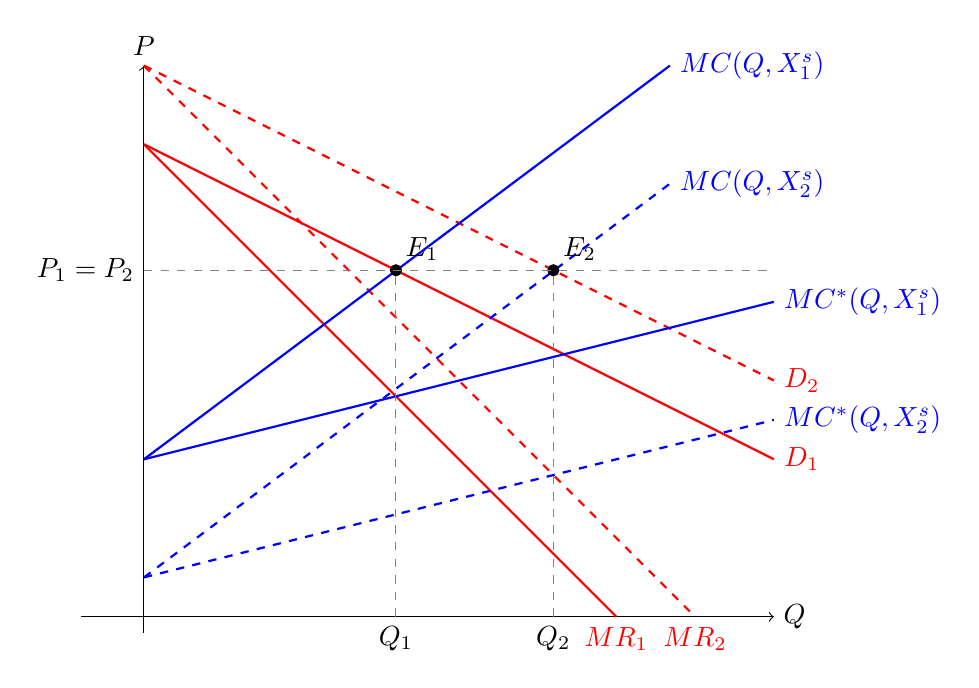
\begin{tikzpicture}[
            x=4cm,   % x軸のスケールを大きく
            y=1cm    % y軸のスケールはそのまま
        ]
            % 座標軸
            \draw[->] (-0.2,0) -- (2,0) node[right] {$Q$};
            \draw[->] (0,-0.2) -- (0,7) node[above] {$P$};
            
            % 需要曲線(傾き-2)
            \draw[red, thick] (0,6) -- (2,2) node[right] {$D_1$};
            \draw[red, thick, dashed] (0,7) -- (2,3) node[right] {$D_2$};
            
            % 限界収入曲線(傾き-4)
            \draw[red, thick] (0,6) -- (1.5,0) node[below] {$MR_1$};
            \draw[red, thick, dashed] (0,7) -- (1.75,0) node[below] {$MR_2$};
            
            % 限界費用曲線(X1_s=1のとき)
            \draw[blue, thick] (0,2) -- (1.67,7) node[right] {$MC(Q,X_1^s)$};
            \draw[blue, thick] (0,2) -- (2,4) node[right] {$MC^*(Q,X_1^s)$};
            
            % 限界費用曲線(X2_s=-0.5のとき)
            \draw[blue, thick, dashed] (0,0.5) -- (1.67,5.5) node[right] {$MC(Q,X_2^s)$};
            \draw[blue, thick, dashed] (0,0.5) -- (2,2.5) node[right] {$MC^*(Q,X_2^s)$};

            % 均衡点(同じ高さ4.4)
            \filldraw[black] (0.8,4.4) circle (2pt) node[above right] {$E_1$};
            \filldraw[black] (1.3,4.4) circle (2pt) node[above right] {$E_2$};
            
            % 補助線
            \draw[gray, dashed] (0.8,0) -- (0.8,4.4);
            \draw[gray, dashed] (1.3,0) -- (1.3,4.4);
            \draw[gray, dashed] (0,4.4) -- (2,4.4);
            
            % ラベル
            \node[below] at (0.8,0) {$Q_1$};
            \node[below] at (1.3,0) {$Q_2$};
            \node[left] at (0,4.4) {$P_1=P_2$};
        \end{tikzpicture}
    \end{center}
    \caption{The illustration of the non-identification result}
    \label{fig:bresnahan_non_transformation}
    \vspace{2mm}
    \footnotesize
    Note: $MC$ is the marginal cost rationalized by the perfect competition, and $MC^{*}$ is the marginal cost rationalized by the perfect competition. $\beta_1^* = \beta_1 - \alpha_1$ holds.
    The perfect competition and the monopoly rationalize the equilibrium point $E_1$. The shift in the demand does not help because the new equilibrium $E_2$ still are rationalized by both models.
\end{figure}





\subsection{The log-linear model}

The simplified version of our example is the following:
\begin{align}
    P & = \exp(\varepsilon_{d}) Q^{-\alpha_0} (X^{d})^{\alpha_1},\label{eq:simple_demand} \\
    MC & = \exp(\varepsilon_{s}) Q^{\beta_0} (X^{s})^{\beta_1}. \label{eq:simple_marginal_cost}
\end{align}
and hence, the marginal revenue is
\begin{align}
    MR = (1- \alpha_0)\exp(\varepsilon_{d}) Q^{-\alpha_0} (X^{d})^{\alpha_1}
\end{align}
Take the logarithm of the demand and the marginal revenue, we have
\begin{align}
    \log P & = -\alpha_0 \log Q + \alpha_1 \log X^{d} + \varepsilon_d,\\
    \log MR& = \log (1 -\alpha_0) -\alpha_0 \log Q + \alpha_1 \log X^{d} + \varepsilon_d.
\end{align}
On the other hand, the supply relation becomes
\begin{align}
    \log P = -\log (1 - \theta \alpha_0) + \beta_0 \log Q + \beta_1 \log X^{s} + \varepsilon_s. \label{eq:simple_supply}
\end{align}

While the conduct parameter changes the slope of the supply relation in Bresnahan's example, the change in the conduct parameter shifts the supply relation in our example.
To make the model feasible, we assume that $1- \theta \alpha_0 >0$ for any $\theta \in [0,1]$.
Because $\alpha_0>0$ and $\theta \in [0,1]$, $1- \theta\alpha_0 <1$, which implies that $- \log(1- \theta\alpha_0) > 0$.
Then, for example, when we compare perfect competition and monopoly,  the supply relations under perfect competition and monopoly are parallel by $\log(1 - \alpha_0)$, and the supply relation under monopoly is shifted upward to the supply relation under perfect competition.

Note also that $\log (1 - \alpha_0)$ parallels the demand function and the marginal revenue, and the marginal revenue is shifted downwards.

Figure \ref{fig:simpe_identification} plots the above equations as in Bresnahan's example.
As we can see, under perfect competition and monopoly, the equilibrium quantities under the two models differ.

and the equilibrium quantity is given by
\begin{align}
    \log Q_t &= \frac{ \log (1 - \theta \alpha_0 ) + \alpha_1 \log X^{d}- \beta_2 \log X^{s} + \varepsilon^{d} - \varepsilon^{c}}{\alpha_0 + \beta_0 }.\label{eq:quantity_loglinear}
\end{align}

\begin{figure}[t]
    \centering
        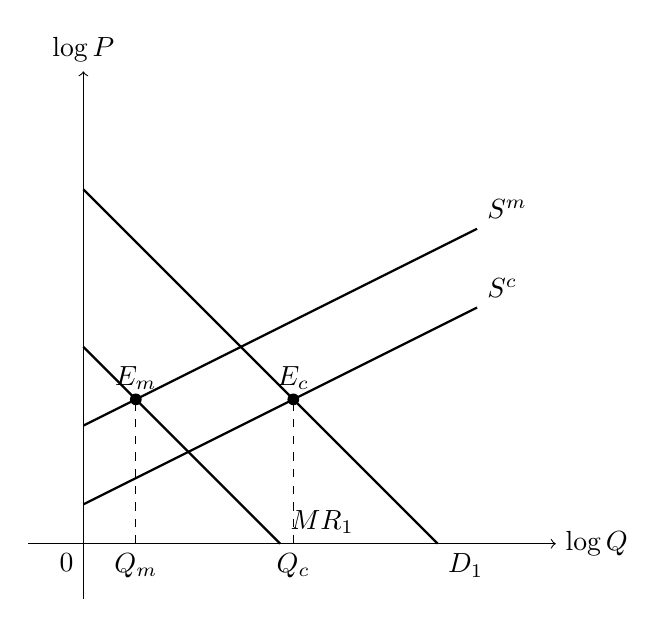
\begin{tikzpicture}
            % Axes
            \draw[->] (-0.7,0) -- (6,0) node[right] {$\log Q$}; % Horizontal axis
            \draw[->] (0,-0.7) -- (0,6) node[above] {$\log P$}; % Vertical axis

            % Marginal Revenue (MR_1) - passes through (0,5), (3,2), and (5,0)
            \draw[thick] (0,4.5) -- (4.5,0) node[below right] {$D_1$};
            \draw[thick] (0,2.5) -- (2.5,0) node[above right] {$MR_1$};
            
            % Supply Curve under competition (S^c) - passes through (0,1), (3,4), and (4.5,5.5)
            \draw[thick] (0,1.5) -- (5,4) node[above right] {$S^m$};
            % Supply Curve under monopoly (S^m) - passes through (0,1), (3,2), and (7.5,3.5)
            \draw[thick] (0,0.5) -- (5,3) node[above right] {$S^c$};

            % Equilibrium point (E_1) - intersection of D_1 and S^c at (3,4)
            \node[circle, fill, inner sep=1.5pt] (Ec) at (2/3,11/6) {};
            \node[above] at (Ec) {$E_m$};

            \node[circle, fill, inner sep=1.5pt] (Em) at (8/3,11/6) {};
            \node[above] at (Em) {$E_c$};
            % Additional labels
            \node[below left] at (0,0) {0};
            \node[below] at (2/3, 0) {$Q_m$};
            \node[below] at (8/3, 0) {$Q_c$};

            \draw[dashed] (8/3,0) -- (8/3,11/6);
            \draw[dashed] (2/3,0) -- (2/3,11/6);
        \end{tikzpicture}
        \caption{}
    \caption{Identification of the conduct under the log-linear model}
    \label{fig:simpe_identification}
\end{figure}








\subsection{The log-linear model}

The simplified version of our example is the following:
\begin{align}
    P & = \exp(\alpha_0) Q^{-\alpha_1} (X^{d})^{\alpha_2},\label{eq:simple_demand} \\
    MC & = \exp(\beta_0) Q^{\beta_1} (X^{s})^{\beta_2}. \label{eq:simple_marginal_cost}
\end{align}
and hence, the marginal revenue is
\begin{align}
    MR = (1- \theta\alpha_1)\exp(\alpha_0) Q^{-\alpha_1} (X^{d})^{\alpha_2}
\end{align}
Take the logarithm of the demand and the marginal revenue, we have
\begin{align}
    \log P & = \alpha_0 -\alpha_1 \log Q + \alpha_2 \log X^{d},\\
    \log MR& = \log (1 -\theta\alpha_1) + \alpha_0 -\alpha_1 \log Q + \alpha_2 \log X^{d}.
\end{align}
The logarithm of the marginal cost is given by
\begin{align}
    \log MC & = \beta_0 + \beta_1 \log Q + \beta_2 \log X^{s}.
\end{align}
The intersection of the marginal revenue and the marginal cost gives the equilibrium log quantity;
\begin{align}
    \log Q &= \frac{ \log (1 - \theta \alpha_1) + \alpha_0 - \beta_0 +\alpha_2 \log X^{d} - \beta_2 \log X^{s}}{\alpha_1 + \beta_1}.
\end{align}
Thus, the equilibrium quantity is given by
\begin{align}
    Q &= \exp\left(\frac{ \log (1 - \theta \alpha_1) + \alpha_0 - \beta_0 +\alpha_2 \log X^{d} - \beta_2 \log X^{s}}{\alpha_1 + \beta_1}\right)\\
    &= \exp(\alpha_0) \left( \frac{1 - \theta \alpha_1}{1 - \alpha_1}\right)^{\frac{\alpha_1}{\alpha_1 + \beta_1}} X^{d\frac{\alpha_2}{\alpha_1 + \beta_1}} X^{s\frac{\beta_2}{\alpha_1 + \beta_1}}.
\end{align}


While the conduct parameter changes the slope of the supply relation in Bresnahan's example, the change in the conduct parameter shifts the supply relation in our example.
To make the model feasible, we assume that $1- \theta \alpha_0 >0$ for any $\theta \in [0,1]$.
Because $\alpha_0>0$ and $\theta \in [0,1]$, $1- \theta\alpha_0 <1$, which implies that $- \log(1- \theta\alpha_0) > 0$.
Then, for example, when we compare perfect competition and monopoly,  the supply relations under perfect competition and monopoly are parallel by $\log(1 - \alpha_0)$, and the supply relation under monopoly is shifted upward to the supply relation under perfect competition.

Note also that $\log (1 - \alpha_0)$ parallels the demand function and the marginal revenue, and the marginal revenue is shifted downwards.

Figure \ref{fig:simpe_identification} plots the above equations as in Bresnahan's example.
As we can see, under perfect competition and monopoly, the equilibrium quantities under the two models differ.

and the equilibrium quantity is given by
\begin{align}
    \log Q_t &= \frac{ \log (1 - \theta \alpha_0 ) + \alpha_1 \log X^{d}- \beta_2 \log X^{s} + \varepsilon^{d} - \varepsilon^{c}}{\alpha_0 + \beta_0 }.\label{eq:quantity_loglinear}
\end{align}



\subsection{Linear Model}

\citet{bresnahan1982oligopoly} considers the following linear demand and linear marginal cost model:
\begin{align}
    P & = \alpha_0 - \alpha_1 Q + \alpha_2 X^d + \varepsilon_d,\label{eq:bresnahan_demand} \\
    MC & = \beta_0 + \beta_1 Q + \beta_2 X^s + \varepsilon_s. \label{eq:bresnahan_marginal_cost}
\end{align}
Assume that $\alpha_1>0$ and $\beta_1 >0$.
The marginal revenue under $\theta$ is
\begin{align}
    MR = \alpha_0 - \alpha_1(1 + \theta) Q + \alpha_2 X^d + \varepsilon_d. \label{eq:bresnahan_marginal_revenue}
\end{align}
Note that when $\theta = 1$, the slope of the marginal revenue is twice as steep as the demand function under a linear demand model.

The first-order condition implies that the intersection between the marginal revenue \eqref{eq:bresnahan_marginal_revenue} and the marginal cost \eqref{eq:bresnahan_marginal_cost} determines the equilibrium quantity.
The other way to get the equilibrium quantity is to use the demand function and the supply function.
Based on the first-order condition, the supply relation can be computed as
\begin{align}
    P & = \beta_0 + (\beta_1 + \theta\alpha_1) Q  + \beta_2 X^s + \varepsilon_s.\label{eq:bresnahan_supply}
\end{align}
The intersection of \eqref{eq:bresnahan_demand} and \eqref{eq:bresnahan_supply} derives the equilibrium price and the equilibrium quantity.
The equilibrium quantity is given by
\begin{align}
    Q^e = \frac{\alpha_0 + \alpha_2 X^d - \beta_0 - \beta_2 X^s + \varepsilon_d - \varepsilon_s}{\alpha_1(1 + \theta) +  \beta_1}.
\end{align}

For a true marginal cost parameter $\beta$ and the conduct parameter $\theta$, consider the marginal cost parameter of the alternative model given by
\begin{align}
    \beta_0^{*} = \beta_0, \quad \beta_1^{*} = \beta_1 + \alpha_1(\theta - \theta^{*}), \quad \beta_2^{*} = \beta_2.
\end{align}
Thus, the marginal cost under the alternative model is different from the true model only in the coefficient of $Q$.
In this case the model with $(\theta, \beta)$ is observationally equivalent to the model with $(\theta^{*}, \beta^{*})$.


In \citet{bresnahan1982oligopoly}, he considers perfect competition ($\theta = 0$) and monopoly ($\theta = 1$).
Assume that the true model is the perfect competition, and then monopoly is the alternative model.
Then, the marginal cost parameter $\beta^{*}$ of the alternative model is given by
\begin{align}
    \beta_0^{*} = \beta_0, \quad \beta_1^{*} = \beta_1 - \alpha_1, \quad \beta_2^{*} = \beta_2.
\end{align}

In this example, the equilibrium quantity in the true model is given by
\begin{align}
    Q = \frac{\alpha_0 + \alpha_2 X^d - \beta_0 - \beta_2 X^s + \varepsilon_d - \varepsilon_s}{\alpha_1 + \beta_1}
\end{align}
The equilibrium quantity in the alternative model is given by
\begin{align}
    Q^{*} = \frac{\alpha_0 + \alpha_2 X^d - \beta_0^{*} - \beta_2^{*} X^s + \varepsilon_d - \varepsilon_s}{2\alpha_1 + \beta_1^{*}}.
\end{align}
Then, by the assumption on $\beta^{*}$, the equilibrium quantity is the same in both models ($Q = Q^{*}$) for any $X^d$ and $X^s$ because the denominator has the same value, and hence, the researcher cannot distinguish two models from the data.

Figure \ref{fig:bresnahan_non_identification} illustrates this situation.
$E_1$ is the observed equilibrium outcome, and both models rationalize the equilibrium.
Furthermore, the demand shift due to the increase of $X^d$ does not help identify the conduct, which equally increases $Q$ and $Q^{*}$, and $E_2$, the new equilibrium point, is still rationalized by both models.
We can also demonstrate that the conduct parameter cannot be identified in the supply relation \eqref{eq:bresnahan_supply}.
Let $\gamma = (\beta_1 + \theta \alpha_1)$.
Then, the parameter can be identified  in \eqref{eq:bresnahan_supply} are $\beta_0$,$\gamma$, and $\beta_2$, but we cannot identify $\theta$ as $\gamma$ in both models has the same value; 
\begin{align}
    \gamma &= \beta_1 + \theta \alpha_1 = \beta_1 = \beta_1 + \alpha_1 = \gamma^{*}.
\end{align}

\begin{figure}
    \begin{center}
        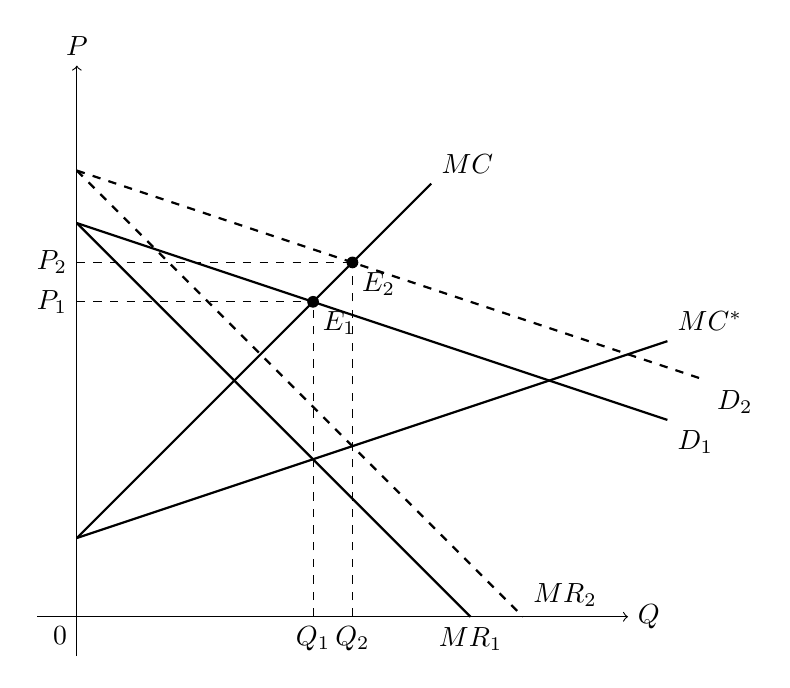
\begin{tikzpicture}
        % Axes
        \draw[->] (-0.5,0) -- (7,0) node[right] {$Q$}; % Horizontal axis
        \draw[->] (0,-0.5) -- (0,7) node[above] {$P$}; % Vertical axis
    
        % Demand Curve (D_1) - passes through (0,5), (3,4), and (7.5,2.5)
        \draw[thick] (0,5) -- (7.5,2.5) node[below right] {$D_1$};
    
        % Marginal Revenue (MR_1) - passes through (0,5), (3,2), and (5,0)
        \draw[thick] (0,5) -- (5,0) node[below] {$MR_1$};
    
        % Supply Curve under competition (S^c) - passes through (0,1), (3,4), and (4.5,5.5)
        \draw[thick] (0,1) -- (4.5,5.5) node[above right] {$MC$};
    
        % Supply Curve under monopoly (S^m) - passes through (0,1), (3,2), and (7.5,3.5)
        \draw[thick] (0,1) -- (7.5,3.5) node[above right] {$MC^{*}$};
    
        % Equilibrium point (E_1) - intersection of D_1 and S^c at (3,4)
        \node[circle, fill, inner sep=1.5pt] (E1) at (3,4) {};
        \node[below right] at (E1) {$E_1$};
    
    
        % Equilibrium point (E_2) - intersection of D_1 and S^c at (7/2,9/2)
        \node[circle, fill, inner sep=1.5pt] (E2) at (7/2,9/2) {};
        \node[below right] at (E2) {$E_2$};
    
        % Shifted Demand Curve (D_1 shifted)
        \draw[thick, dashed] (0,34/6) -- (8,3) node[below right] {$D_2$};
        
        % Shifted MR (MR_1 shifted)
        \draw[thick, dashed] (0,34/6) -- (34/6,0) node[above right] {$MR_2$};
        
        % Dashed lines for price and quantity
        \draw[dashed] (3,0) -- (3,4);
        \draw[dashed] (0,4) -- (3,4);
    
        \draw[dashed] (0,9/2) -- (7/2,9/2);
        \draw[dashed] (7/2,0) -- (7/2,9/2);
    
        % Additional labels
        \node[below left] at (0,0) {0};
        \node[left] at (0,4) {$P_1$};
        \node[below] at (3,0) {$Q_1$};
    
        \node[left] at (0,9/2) {$P_2$};
        \node[below] at (7/2,0) {$Q_2$};
    \end{tikzpicture}
    \end{center}
    \caption{The illustration of the non-identification result}
    \label{fig:bresnahan_non_identification}
    \vspace{2mm}
    \footnotesize
    Note: $MC$ is the marginal cost rationalized by the perfect competition, and $MC^{*}$ is the marginal cost rationalized by the perfect competition. $\beta_c = \beta_m + \alpha_1$ holds.
    The perfect competition and the monopoly rationalize the equilibrium point $E_1$. The shift in the demand does not help because the new equilibrium $E_2$ still are rationalized by both models.
\end{figure}


Let's investigate the same model with Lau's argument.
As Figure \ref{fig:bresnahan_non_identification} shows, the demand function and the marginal revenue with $\theta = 1$ have different slopes.
$MC$ and $MC^{*}$ are also different in the slope.
\begin{align}
    (1+\theta) \frac{\partial P}{\partial Q}(Q, X^d) + \theta \frac{\partial^2 P}{\partial Q^2}(Q, X^d) Q  - \frac{\partial MC}{\partial Q}(Q, X^s) = -\alpha_1(1 + \theta)   - \beta_1.
\end{align}
Due to the assumption on the marginal cost parameter between $MC$ and $MC^{*}$,
\begin{align}
    \lambda(X^{d}, X^{s}) = \frac{-2\alpha_1  - \beta_1^{*}}{-\alpha_1  - \beta_1} =   \frac{-2\alpha_1  -\beta_1 + \alpha_1}{-\alpha_1  - \beta_1} = 1.
\end{align}

The numerator of \eqref{eq:derivative_q_x_d} is given by
\begin{align}
    \frac{\partial P}{\partial X^{d}}(Q, X^{d}) + \theta\frac{\partial^2 P}{\partial X^{d}\partial Q}(Q, X^{d})Q   = \alpha_2
\end{align}
and the numerator of \eqref{eq:derivative_q_x_s} is given by
\begin{align}
    \frac{\partial MC}{\partial X^{s}}(Q, X^{s}) = \beta_2.
\end{align}
Then, \eqref{eq:derivative_q_x_d} and \eqref{eq:derivative_q_x_s} are 
\begin{align}
    \frac{\partial h}{\partial X^{d}}(Q, X^{d}) = \frac{\partial h^{*}}{\partial X^{d}}(Q, X^{d})  = \frac{\alpha_2}{\alpha_1 + \beta_1},\\
    \frac{\partial h}{\partial X^{s}}(Q, X^{s}) = \frac{\partial h^{*}}{\partial X^{s}}(Q, X^{s})  =-\frac{\beta_2}{\alpha_1 + \beta_1}.
\end{align}
which implies that observable equivalence holds for any $X^d$ and $X^s$.


By applying Lemma \ref{lemma_1_GU}, we can say that there is a transformation $T$ such that
\begin{align}
    P(Q, X^d) + \frac{\partial P}{\partial Q}(Q, X^d) Q & = T(P(Q, X^d), Q)\\
    MC^{*}(Q, X^s) &= T(MC(Q, X^s), Q).
\end{align}
In this case, consider the following transformation:
\begin{align}
    T(x, Q) = x + \alpha_1(\theta - \theta^{*})Q.
\end{align}
Then, we have
\begin{align}
    T(MC(Q, X^s), Q) & =  \beta_0 + \beta_1 Q + \beta_2 X^s + \alpha_1(\theta - \theta^{*})Q\\
    & = \beta_0^{*} + \beta_1^{*} Q + \beta_2^{*} X^s\\
    & = MC^{*}(Q, X^s).
\end{align}
and
\begin{align}
    T\left(P(Q, X^d) + \theta \frac{\partial P}{\partial Q}(Q, X^d) Q, Q\right) & = P(Q, X^d) -\theta \alpha_1 Q +  \alpha_1(\theta - \theta^{*})Q\\ 
    & = P(Q, X^d) - \theta^{*} \alpha_1 Q  \\
    & = P(Q, X^d) + \theta^{*} \frac{\partial P}{\partial Q}(Q, X^d) Q.
\end{align}

\subsection{The log-linear model}
The simplified version of our example is the following:
\begin{align}
    P & = \exp(\alpha_0) Q^{-\alpha_1} (X^{d})^{\alpha_2}, \\
    MC & = \exp(\beta_0) Q^{\beta_1} (X^{s})^{\beta_2}.
\end{align}
and hence, the marginal revenue is
\begin{align}
    MR = (1- \theta\alpha_1)\exp(\alpha_0) Q^{-\alpha_1} (X^{d})^{\alpha_2}
\end{align}
Take the logarithm of the demand and the marginal revenue, we have
\begin{align}
    \log P & = \alpha_0 -\alpha_1 \log Q + \alpha_2 \log X^{d},\\
    \log MR& = \log (1 -\theta\alpha_1) + \alpha_0 -\alpha_1 \log Q + \alpha_2 \log X^{d}.
\end{align}
The logarithm of the marginal cost is given by
\begin{align}
    \log MC & = \beta_0 + \beta_1 \log Q + \beta_2 \log X^{s}.
\end{align}
The intersection of the marginal revenue and the marginal cost gives the equilibrium log quantity;
\begin{align}
    \log Q &= \frac{ \log (1 - \theta \alpha_1) + \alpha_0 - \beta_0 +\alpha_2 \log X^{d} - \beta_2 \log X^{s}}{\alpha_1 + \beta_1}.
\end{align}
Thus, the equilibrium quantity is given by
\begin{align}
    Q^e &= \left[(1 - \theta \alpha_1)\exp(\alpha_0 - \beta_0)\right]^{\frac{1}{\alpha_1 + \beta_1}} (X^{d})^{\frac{\alpha_2}{\alpha_1 + \beta_1}} (X^{s})^{\frac{\beta_2}{\alpha_1 + \beta_1}}.
\end{align}
Based on the equilibrium quantity, consider an alternative model where the marginal cost function is defined as
\begin{align}
    MC^{*}(Q, X^{s}) = \exp(\beta_0^*) Q^{\beta_1^*} (X^{s})^{\beta_2^*}
\end{align}
where 
\begin{align}
    \beta_0^* = \beta_0 + \log\left(\frac{1-\theta^*\alpha_1}{1 - \theta\alpha_1}\right),\quad\beta_1^* = \beta_1,\quad \beta_2^* = \beta_2.
\end{align}
Then, between the true model and the alternative model, we have 
\begin{align}
    \lambda(Q, X^{s}) & = \frac{(1 -\theta\alpha_1)\alpha_1 \exp(\alpha_0) Q^{-\alpha_1 - 1}(X^{d})^{\alpha_2} - \beta_1 \exp(\beta_0)Q^{\beta_1-1} (X^{s})^{\beta_2}}{(1 -\theta^{*}\alpha_1)\alpha_1 \exp(\alpha_0) Q^{-\alpha_1 - 1}(X^{d})^{\alpha_2} - \beta_1^{*} \exp(\beta_0^{*})Q^{\beta_1^{*}-1} (X^{s})^{\beta_2^{*}}} \\
    & = \frac{(1 -\theta\alpha_1)\alpha_1 \exp(\alpha_0) Q^{-\alpha_1 - 1}(X^{d})^{\alpha_2} - \beta_1 \exp(\beta_0)Q^{\beta_1-1} (X^{s})^{\beta_2}}{(1 -\theta^{*}\alpha_1)\alpha_1 \exp(\alpha_0) Q^{-\alpha_1 - 1}(X^{d})^{\alpha_2} - \beta_1 \exp(\beta_0)\left(\frac{1-\theta^*\alpha_1}{1 - \theta\alpha_1}\right)   Q^{\beta_1-1} (X^{s})^{\beta_2}} \\
    & = \left(\frac{1-\theta^*\alpha_1}{1 - \theta\alpha_1}\right).
\end{align}
Thus, the transformation can be defined as
\begin{align}
    T(x, Q) = \frac{1 - \theta^* \alpha_1}{1 - \theta \alpha_1}x.
\end{align}
In fact, under the transformation, we have
\begin{align}
    T\left(P(Q, X^{d}) + \theta \frac{\partial P}{\partial Q}(Q, X^{d}) Q, Q\right)
    &= \frac{1 - \theta^*\alpha_1}{1- \theta\alpha_1} (1 - \theta\alpha_1)\exp(\alpha_0) Q^{-\alpha_1} (X^{d})^{\alpha_2}\\
    & = (1 - \theta^{*}\alpha_1)\exp(\alpha_0) Q^{-\alpha_1} (X^{d})^{\alpha_2}\\
    &= P(Q, X^{d}) + \theta^{*} \frac{\partial P}{\partial Q}(Q, X^{d}) Q
\end{align}
and
\begin{align}
    T\left(MC(Q, X^{s}), Q\right) &= \frac{1 - \theta^*\alpha_1}{1- \theta\alpha_1}\exp(\beta_0) Q^{\beta_1} (X^{s})^{\beta_2}\\
    &= \exp\left(\beta_0 + \log\left(\frac{1 - \theta^*\alpha_1}{1- \theta\alpha_1}\right)\right) Q^{\beta_1} (X^{s})^{\beta_2}\\
    &= MC^{*}(Q, X^{s}).
\end{align}
Thus, $(\theta, MC)$ and $(\theta^{*}, MC^{*})$ are observably equivalent.



\end{document}